% !TeX program = xelatex
\documentclass[12pt, a4paper, twoside, reqno]{article}

\def\history{Published 2026/08/25}
\def\chistory{出版日期：2026年8月25日}

%%
%% This is file `SCAM-ctemplate.sty' used for Chinese Project Report of Students
%% in Department of Smart Computing and Applied Mathematicsm TUnghai Univsersity
%%
%% Copyright 2026/6/22
%%
%% The LaTeX3 Project and any individual authors listed elsewhere
%% in this file.
%%
%% This file was generated from file(s) of the LaTeX base system.
%% --------------------------------------------------------------
%%
%% It may be distributed and/or modified under the
%% conditions of the LaTeX Project Public License, either version 1.3c
%% of this license or (at your option) any later version.
%% The latest version of this license is in
%%    http://www.latex-project.org/lppl.txt
%% and version 1.3c or later is part of all distributions of LaTeX
%% version 2005/12/01 or later.
%%
%% This file has the LPPL maintenance status "maintained".
%%
%% This file may only be distributed together with a copy of the LaTeX
%% base system. You may however distribute the LaTeX base system without
%% such generated files.
%%
%% The list of all files belonging to the LaTeX base distribution is
%% given in the file `manifest.txt'. See also `legal.txt' for additional
%% information.
%%
%% The list of derived (unpacked) files belonging to the distribution
%% and covered by LPPL is defined by the unpacking scripts (with
%% extension .ins) which are part of the distribution.
%% \CharacterTable
%%  {Upper-case    \A\B\C\D\E\F\G\H\I\J\K\L\M\N\O\P\Q\R\S\T\U\V\W\X\Y\Z
	%%   Lower-case    \a\b\c\d\e\f\g\h\i\j\k\l\m\n\o\p\q\r\s\t\u\v\w\x\y\z
	%%   Digits        \0\1\2\3\4\5\6\7\8\9
	%%   Exclamation   \!     Double quote  \"     Hash (number) \#
	%%   Dollar        \$     Percent       \%     Ampersand     \&
	%%   Acute accent  \'     Left paren    \(     Right paren   \)
	%%   Asterisk      \*     Plus          \+     Comma         \,
	%%   Minus         \-     Point         \.     Solidus       \/
	%%   Colon         \:     Semicolon     \;     Less than     \<
	%%   Equals        \=     Greater than  \>     Question mark \?
	%%   Commercial at \@     Left bracket  \[     Backslash     \\
	%%   Right bracket \]     Circumflex    \^     Underscore    \_
	%%   Grave accent  \`     Left brace    \{     Vertical bar  \|
	%%   Right brace   \}     Tilde         \~}


%
%-----------------------------------------------------------------------
% The 2-3 digits of article number denote area of paper, i.e., 01 math, 02 phy,
% 03 chem, 04 life science, we can add on and keep it here
%-----------------------------------------------------------------------
% \def\articleID{10001}
% \def\doino{10.29273/TS.202307\_24.} 
\def\JournalName{Project Report(2026)}
\def\cJournalName{專題研究報告(2026)}

\usepackage[numbers,compress]{natbib}
\usepackage{url}
\usepackage[no-math]{fontspec}
%
% use font Times for math and text
%
\usepackage{mathptmx}
\usepackage{amsmath, amsthm, amssymb, mathrsfs}
\DeclareSymbolFontAlphabet{\mathcal}{symbols}
\DeclareMathAlphabet{\mathcal}{OMS}{cmsy}{m}{n}
\SetMathAlphabet\mathcal{bold}{OMS}{cmsy}{bx}{n}
\usepackage{tocbibind} % add bibiography into pdf's bookmark

\usepackage[dvipsnames, svgnames, table]{xcolor} %引用顏色套件
\usepackage{colortbl} % \setlength\minrowclearance{2.4pt}
\usepackage{array}
\usepackage{float}
\usepackage{calc}
\usepackage{graphicx}
\DeclareGraphicsExtensions{.pdf, .PDF, .png, .PNG, .jpg, .JPG, .JPEG}
\usepackage{tikz,pgfplots}
\pgfplotsset{compat=1.16}
\pagestyle{empty}
\setcounter{tocdepth}{1}

\usepackage[unicode=true,
 bookmarks=true, bookmarksnumbered=false, bookmarksopen=true, bookmarksopenlevel=3,
 breaklinks=false,
 pdfborder={0 0 0},pdfborderstyle={},
%-----------------------------------------------------------------------
% 參考文獻的引用的頁碼，最後版本將下行關掉，
%-----------------------------------------------------------------------
% backref=page,
%-----------------------------------------------------------------------
% 取消 footnote 的hyperlink
%-----------------------------------------------------------------------
hyperfootnotes=false,
colorlinks=true]
{hyperref}


\makeatletter

%%%%%%%%%%%%%%%%%%%%%%%%%%%%%% LyX specific LaTeX commands.
%% Because html converters don't know tabularnewline
\providecommand{\tabularnewline}{\\}

%%%%%%%%%%%%%%%%%%%%%%%%%%%%%% Textclass specific LaTeX commands.
\theoremstyle{plain}
\newtheorem{thm}{\protect\theoremname}

\@ifundefined{date}{}{\date{}}

%
%page dimensions
%
\setlength    {\textheight}      {22.7cm}
\setlength    {\textwidth}       {15.4cm}
\setlength    {\topmargin}       {-1cm}
\setlength    {\headheight}      {0.5cm}
\setlength    {\headsep}         {0.75cm}
\setlength    {\oddsidemargin}   {0.5cm}
\setlength    {\evensidemargin}  {0.5cm}
\renewcommand {\baselinestretch} {1.25}

%\setlength    {\footskip}        {1cm}
%\setlength    {\footheight}      {0.4cm}
%\setlength    {\parskip}         {0.1cm}
%\setlength    {\baselineskip}    {0.4cm}
%\setlength    {\parindent}       {5ex}
%\setlength {\topsep} {0cm}
% ----------------------------------------------------------------------
%
% control flags
% ----------------------------------------------------------------------
\makeatletter
%-----------------------------------------------------------------------
%
% 設定中文計數
% ----------------------------------------------------------------------
% CAlph
\newcount\c@iv \newcount\c@iii \newcount\c@ii \newcount\c@i \newcount\c@tmp
\def\CAlph#1{\expandafter\@CAlph\csname c@#1\endcsname}
\def\@CAlph#1{%
	\ifcase#1\or 壹\or 貳\or 參\or 肆\or 伍\or 陸\or 柒\or 捌\or 玖\or 拾
	\else\@IcAlph{#1}\fi}
\def\@IcAlph#1{%
	\ifcase#1\or\or\or\or\or\or\or\or\or\or
	\or 拾壹\or 拾貳\or 拾參\or 拾肆\or 拾伍\or 拾陸\or 拾柒\or 拾捌\or 拾九\or
	貳拾\or 貳拾壹\or 貳拾貳\or 貳拾參\or 貳拾肆\or 貳拾伍\or 貳拾陸\or 貳拾柒\or
	貳拾捌\or 貳拾玖
	\else\@IIcAlph{#1}\fi}
\def\@IIcAlph#1{%
	\c@ii=#1\divide\c@ii by10
	\c@tmp=\c@ii\multiply\c@tmp by10
	\c@i=#1\advance\c@i by-\c@tmp
	\ifcase\c@ii\or\or\or 參拾\or 肆拾\or 伍拾\or 陸拾\or 柒拾\or 捌拾\or 九拾
	\else\@IIIcAlph{\c@ii}{\c@i}\fi
	\ifcase\c@i\or 壹\or 貳\or 參\or 肆\or 伍\or 陸\or 柒\or 捌\or 玖
	\fi}
\def\@IIIcAlph#1#2{%
	\c@iii=#1\divide\c@iii by10
	\c@tmp=\c@iii\multiply\c@tmp by10
	\c@ii=#1\advance\c@ii by-\c@tmp
	\ifcase\c@iii\or 一佰\or 二佰\or 三佰\or 四佰\or 五佰\or 六佰\or 七佰\or 八佰\or 九佰
	\else\@IVcAlph{\c@iii}{\c@ii}\fi
	\ifnum\c@ii=0\ifnum#2>0零\fi\else
	\ifcase\c@ii\or 壹\or 貳\or 參\or 肆\or 伍\or 陸\or 柒\or 捌\or 玖\or 拾}
\def\@IVcAlph#1#2{%
	\c@iv=#1\divide\c@iv by10
	\c@tmp=\c@iv\multiply\c@tmp by10
	\c@iii=#1\advance\c@iii by-\c@tmp
	\ifcase\c@iv\or 壹\or 貳\or 參\or 肆\or 伍\or 陸\or 柒\or 捌\or 玖
	\else\@ctrerr\fi
	千\ifnum\c@iii=0\ifnum#2>0零\fi
	\else\ifcase\c@iii\or 壹\or 貳\or 參\or 肆\or 伍\or 陸\or 柒\or 捌\or 玖\fi 百\fi}
% Calph
\newcount\c@iv \newcount\c@iii \newcount\c@ii \newcount\c@i \newcount\c@tmp
\def\Calph#1{\expandafter\@Calph\csname c@#1\endcsname}
\def\@Calph#1{%
   \ifcase#1\or 一\or 二\or 三\or 四\or 五\or 六\or 七\or 八\or 九\or 十
   \else\@Icalph{#1}\fi}
\def\@Icalph#1{%
   \ifcase#1\or\or\or\or\or\or\or\or\or\or
   \or 十一\or 十二\or 十三\or 十四\or 十五\or 十六\or 十七\or 十八\or 十九\or
       二十\or 二十一\or 二十二\or 二十三\or 二十四\or 二十五\or 二十六\or 二十七\or
       二十八\or 二十九
   \else\@IIcalph{#1}\fi}
\def\@IIcalph#1{%
   \c@ii=#1\divide\c@ii by10
   \c@tmp=\c@ii\multiply\c@tmp by10
   \c@i=#1\advance\c@i by-\c@tmp
   \ifcase\c@ii\or\or\or 三十\or 四十\or 五十\or 六十\or 七十\or 八十\or 九十
   \else\@IIIcalph{\c@ii}{\c@i}\fi
   \ifcase\c@i\or 一\or 二\or 三\or 四\or 五\or 六\or 七\or 八\or 九
   \fi}
\def\@IIIcalph#1#2{%
   \c@iii=#1\divide\c@iii by10
   \c@tmp=\c@iii\multiply\c@tmp by10
   \c@ii=#1\advance\c@ii by-\c@tmp
   \ifcase\c@iii\or 一百\or 二百\or 三百\or 四百\or 五百\or 六百\or 七百\or 八百\or 九百
   \else\@IVcalph{\c@iii}{\c@ii}\fi
   \ifnum\c@ii=0\ifnum#2>0零\fi\else
   \ifcase\c@ii\or 一\or 二\or 三\or 四\or 五\or 六\or 七\or 八\or 九\fi 十\fi}
\def\@IVcalph#1#2{%
   \c@iv=#1\divide\c@iv by10
   \c@tmp=\c@iv\multiply\c@tmp by10
   \c@iii=#1\advance\c@iii by-\c@tmp
   \ifcase\c@iv\or 一\or 二\or 三\or 四\or 五\or 六\or 七\or 八\or 九
   \else\@ctrerr\fi
  千\ifnum\c@iii=0\ifnum#2>0零\fi
  \else\ifcase\c@iii\or 一\or 二\or 三\or 四\or 五\or 六\or 七\or 八\or 九\fi 百\fi}

% ----------------------------------------------------------------------
% page header and footer
% ----------------------------------------------------------------------
% Definition of 'myheadings' page style.
%
\def\blfootnote{\gdef\@thefnmark{}\@footnotetext}

\def\ps@myheadings
{  \let\@mkboth\@gobbletwo
   \def\@oddhead{\rm
       \vtop{\centering \par\vspace{1ex plus 3ex minus 3ex}
       \rightmark}
       \hspace{0em plus 1em minus 2em}  \hfill \thepage
       }%
   \def\@oddfoot{}
   \def\@evenhead{\rm
       \thepage\hfil \hspace{0em plus 1em minus 2em}
       \vtop{\centering\par\vspace{1ex plus 3ex minus 3ex} \leftmark}
       }%
   \def\@evenfoot{}
   \def\sectionmark##1{}\def\subsectionmark##1{}
}
%
% this page style and make title header for English
%
% need to specify the
\def\ps@thisheadings
{  \let\@mkboth\@gobbletwo
   \def\@oddhead{\rm \JournalName \hfill \thepage}%
   \def\@oddfoot{}
   \def\@evenhead{\rm \thepage \hfill \JournalName}%
   \def\@evenfoot{}
}

\def\abstract{\footnotesize\vspace{1ex}\null
\begin{center}
\blfootnote{~\chistory}
{\large\bf \abstractname \vspace{1.5ex}}
\end{center}
\quotation
}
%
% this page style and make title header for Chinese
%
% need to specify the
% inside the CJK environment
%
\def\ps@cthisheadings
{  \let\@mkboth\@gobbletwo
   \def\@oddhead{\rm \cJournalName
       \hspace{0em plus 2em minus 3em}  \hfill \thepage
   }%
   \def\@oddfoot{}
   \def\@evenhead{\rm \thepage\hfil }%
   \def\@evenfoot{}
   \let\thefootnote\relax
}
\def\@maketitle{\newpage \null
{\centering
	{\LARGE\bfseries\textbf{\@title} \par}     % Title set in \LARGE size.
		\vskip 1ex                    % Vertical space after title. 
		{\Large                       % each author set in \large, in a
			\lineskip .5ex            % tabular environment
			\begin{tabular}[t]{c}\@author
			\end{tabular}\par}
	} \vspace{2ex} \null
}

%
% change the length of the ruler for footnotetext
% the specification of
%   \footnotemark[?}\thanks{...}
% inside title or author, need to move it to a new
% \footnotetext[?]{...}
%
% specify the footnote mark as symbol
%
\renewcommand\footnoterule{%
  \kern-3\p@
  \hrule\@width1.01\columnwidth
  \kern2.6\p@}

\renewcommand\@makefntext[1]{%
    \parindent 1em%
    \noindent
    \hb@xt@0.5em{\hss\@makefnmark}#1}

\renewcommand{\thefootnote}{\fnsymbol{footnote}}

%
% section head information
%
%\def\section{\setcounter{equation}{0}\@startsection {section}{1}{\z@}{6.5ex plus 1ex minus
%    .2ex}{4ex plus .2ex}{\Large\bf\centering}}
%\def\subsection{\@startsection{subsection}{2}{\z@}{0.1ex plus .1ex minus%
%.1ex}{0.1ex plus .1ex}{\large\bf}}
%\def\subsubsection{\@startsection{subsubsection}{3}{\z@}{0.1ex plus .1ex minus%
%.1ex}{0.1ex plus .1ex}{\normalsize\bf}}
\usepackage{titlesec}
\titleformat{\section}{\setcounter{equation}{0}\Large\bfseries\raggedright}{\CAlph{section}、}{0.1em}{}
\titleformat{\subsection}{\large\bfseries\raggedright}{\Calph{subsection}、}{0.1em}{}
\titleformat{\subsubsection}{\bfseries\raggedright}{(\Calph{subsubsection})}{0.1em}{}

% Consistent academic spacing for headings, paragraphs, displays, and bibliography.
\titlespacing{\section}{0pt}{3.2ex plus 0.6ex minus 0.2ex}{1.6ex plus 0.2ex}
\titlespacing{\subsection}{0pt}{2.8ex plus 0.5ex minus 0.2ex}{1.2ex plus 0.2ex}
\titlespacing{\subsubsection}{0pt}{2.4ex plus 0.4ex minus 0.2ex}{0.9ex plus 0.2ex}

\setlength{\parindent}{2em}
\setlength{\parskip}{0pt plus 0.2ex}
\setlength{\abovedisplayskip}{0.75\baselineskip plus 0.2\baselineskip minus 0.15\baselineskip}
\setlength{\belowdisplayskip}{0.75\baselineskip plus 0.2\baselineskip minus 0.15\baselineskip}
\setlength{\abovedisplayshortskip}{0.5\baselineskip plus 0.15\baselineskip}
\setlength{\belowdisplayshortskip}{0.5\baselineskip plus 0.15\baselineskip}
\setlength{\jot}{3pt}
\setlength{\bibhang}{2em}
\setlength{\bibsep}{0pt plus 0.2ex}
\setlength{\emergencystretch}{1em}
\widowpenalty=10000
\clubpenalty=10000
\displaywidowpenalty=10000
\raggedbottom
\titleformat{\subsubsubsection}{\bfseries\raggedright}{\arabic{subsubsubsection}.}{0.1em}{}
\titleformat{\subsubsubsubsection}{\raggedright}{\indent(\arabic{subsubsubsubsection})}{0.1em}{}

%

% ----------------------------------------------------------------------
%  中文定理名稱設定 
% environment for theorem like environment writing.
% ----------------------------------------------------------------------

%
\newtheorem {definition}{定義}[section]
\newtheorem {defn}      {定義}[section]
\newtheorem {example}    [definition]{範例}
\newtheorem {lemma}      [definition]{引理}
\newtheorem {lem}        [definition]{引理}
\newtheorem {theorem}    [definition]{定理}
\newtheorem {problem}    [definition]{問題}
\newtheorem {proposition}[definition]{命題}
\newtheorem {corollary}  [definition]{推論}
\providecommand{\theoremname}{定理}

\newcounter{remark}[section]
\newenvironment{remark} {\stepcounter{definition}\setcounter{remark}{\value{definition}}\vspace{.5em}\par\noindent%
{\bf Remark \theremark}~\begingroup}{\endgroup}
\renewcommand{\theremark}{\thesection.\arabic{remark}~}

%\newcounter{example}[section]
%\newenvironment{example} {\stepcounter{definition}\setcounter{example}{\value{definition}}\vspace{.5em}\par\noindent%
%\textbf{範例 \theexample}~\begingroup\Kai}{\endgroup}
%\renewcommand{\theexample}{\thesection.\arabic{example}.~}

%
% specify the display style for equation number
%
\renewenvironment{proof}[1][\proofname]{\par%
\pushQED{\qed}%
\normalfont \topsep6\p@\@plus6\p@\relax%
\trivlist%
\item[\hskip\labelsep%
#1]\ignorespaces%
}{%
\popQED\endtrivlist\@endpefalse%
}

\makeatother
\renewcommand{\theequation}{\thesection.\arabic{equation}}
\renewcommand{\abstractname}{摘\quad{}要}
\renewcommand{\refname}{參考文獻}
\renewcommand{\tocbibname}{參考文獻}
\renewcommand{\settocname}{參考文獻}
\renewcommand{\appendixname}{附錄}
\renewcommand{\figurename}{圖}
\renewcommand{\tablename}{表}
\renewcommand{\proofname}{\bfseries 證明:}
\renewcommand\contentsname{\bfseries - 目 錄 }
\renewcommand{\listfigurename}{\bfseries 圖 目 錄} 
\renewcommand{\listtablename}{\bfseries 表 目 錄}


% ----------------------------------------------------------------------------
\providecommand{\tabularnewline}{\\}

\newcommand{\noun}[1]{\textsc{#1}}
\makeatother

\usepackage{mathdots, mathtools} % 引用常見的數學符號與設定
\usepackage{bm} % 粗體數學
\usepackage{float} % 固定圖表位置
\usepackage{amsmath}
\definecolor{LightGray}{gray}{0.9}
%%%%%%%%%%%%%%%%%%%%%%%%%%%%%% User specified LaTeX commands.
% ------------------------------- 設定 XeTeX -----------------------------------
\XeTeXlinebreaklocale "zh" %以中文方式斷行 
\XeTeXlinebreakskip = 0pt plus 1pt minus 0.1pt %在字元間加入0pt-1pt使文件左右對齊 
\usepackage{xunicode,xltxtra} 
\usepackage{xeCJK}        %讓中英文字體分開設置
\setmainfont{TeX Gyre Termes}

\setCJKmainfont[
    Path = {./fonts/},                 % Update this to your actual folder path
    BoldFont = {MSJH.TTC},             % Uses for bold text
    BoldFeatures = {FontIndex = 0},    % Targets the primary style inside MSJH.TTC
    ItalicFont = {KAIU.TTF}            % Uses KaiU (標楷體) for italic text
]{MINGLIU.TTC}                         % Uses MingLiU as the base font
\newCJKfontfamily\Kai[
    Path = {./fonts/}, % Remove this line if KAIU.TTF is in the same folder as your .tex file
    AutoFakeBold = 2
]{KAIU.TTF}                         % 標楷體
\newCJKfontfamily\Hei[
    Path = {./fonts/} % Remove this line if KAIU.TTF is in the same folder as your .tex file
]{MSJH.TTC}                         % 黑體
\newCJKfontfamily\Ming[
    Path = {./fonts/} % Remove this line if KAIU.TTF is in the same folder as your .tex file
]{MINGLIU.TTC}                      % 明體

\makeatletter

%%%%%%%%%%%%%%%%%%%%%%%%%%%%%% LyX specific LaTeX commands.
\pdfpageheight\paperheight
\pdfpagewidth\paperwidth

\floatstyle{ruled}
\newfloat{algorithm}{tbp}{loa}
\providecommand{\algorithmname}{演算法}
\floatname{algorithm}{\protect\algorithmname}
\makeatother

\renewcommand{\baselinestretch}{1.4}

%設定圖的存放位置
\graphicspath{{./Pictures/}}
\hypersetup{pdftitle={Runge Phenomena for Equally Spaced Polynomial Interpolation},
	pdfauthor={Huang-Nan Huang},
	pdfkeywords={Runge phenomena, Chebyshev polynomial, polynomial interpolation, complex integration}}
\pagestyle{myheadings}

\usepackage{matlab-prettifier}
\usepackage{braket} %量子符號設定
\setcounter{secnumdepth}{3} %子集設定
\setcounter{tocdepth}{3} %子集設定

% 統一頁碼於頁尾中央；保留既有頁首文字
\makeatletter
\def\ps@myheadings{%
%
  \def\@oddhead{\rm\rightmark\hfill}%
  \def\@evenhead{}%
  \def\@oddfoot{\hfil\csname thepage\endcsname\hfil}%
  \def\@evenfoot{\hfil\csname thepage\endcsname\hfil}%
  \def\sectionmark##1{}\def\subsectionmark##1{}%
}
\def\ps@thisheadings{%
%
  \def\@oddhead{\rm\JournalName\hfill}%
  \def\@evenhead{\rm\hfill\JournalName}%
  \def\@oddfoot{\hfil\csname thepage\endcsname\hfil}%
  \def\@evenfoot{\hfil\csname thepage\endcsname\hfil}%
}
\def\ps@cthisheadings{%
%
  \def\@oddhead{\rm\cJournalName\hfill}%
  \def\@evenhead{}%
  \def\@oddfoot{\hfil\csname thepage\endcsname\hfil}%
  \def\@evenfoot{\hfil\csname thepage\endcsname\hfil}%
%
}
\def\ps@plain{%
%
  \def\@oddhead{}\def\@evenhead{}%
  \def\@oddfoot{\hfil\csname thepage\endcsname\hfil}%
  \def\@evenfoot{\hfil\csname thepage\endcsname\hfil}%
}
\makeatother
\pagestyle{myheadings}

\begin{document}
\lstset{style=Matlab-editor,basicstyle=\linespread{0.8} \mlttfamily}
\lstMakeShortInline " % set the "..." to enclosed inline Matlab commands


\begin{titlepage}
\csname thispagestyle\endcsname{empty}
        \centering
        \vspace*{0.08\textheight}
        %東海大學log
        
\includegraphics[width=0.35\textwidth]{logos/THU_math_logo2.png}
        \vspace*{1.2cm}

        %中文題目
        {\Large\bfseries\Kai Bell型不等式研究 \par}
        \vspace{1.0cm}

        %作者
        {\large\Kai 李士宏\par}
        \vspace{0.8cm}
        %指導教授
        {\large\Kai 指導教授：陳宏益$~$教授\par}

        %日期
        \vfil
        {\large\Kai 中華民國 115年 8月\par}
        \vspace*{0.06\textheight}

\end{titlepage}
\thispagestyle{cthisheadings}



\addcontentsline{toc}{section}{摘要} 
\begin{abstract}
    Bell 不等式\cite{Bell1964}是檢驗量子非定域性的重要工具，其中 $I_{2222}$不等式\cite{CHSH1969}為最基本的形式，而$I_{3322}$不等式\cite{Collins2004,Guo2021}則基於$I_{2222}$基礎上各增加一組測量設定，可用來檢驗更廣泛的量子關聯。本研究利用 Python 數值模擬，比較$I_{2222}$與 $I_{3322}$不等式在純糾纏態\cite{Nielsen2010}、白噪音環境及噪聲通道\cite{Ruan2018}下的量子違背特性。研究首先建立雙量子位元糾纏態，並將測量設定以一般化 Bloch 球面向量\cite{Nielsen2010}表示，透過偏微分求取$I_{2222}$與 $I_{3322}$不等式的最大違背值及最佳測量角度且固定，比較在不同糾纏程度與噪聲參數下的變化。研究發現在部分參數區域中存在不能違背$I_{2222}$不等式的量子態但能違背$I_{3322}$不等式，說明較多的測量設定\cite{Brunner2008}在特定條件下能辨識出不同的量子非定域性；然而在部分高噪聲環境下，$I_{2222}$不等式展現較佳的魯棒性\cite{Brunner2008}。
	\medskip{}
	
	\par
本專題報告旨在回顧與探討 $I_{2222}$ 與 $I_{3322}$ 模型的相關理論，奠基於文獻~\cite{Collins2004,Guo2021} 的研究基礎，並對其核心理論進行系統性梳理。本研究的主要貢獻在於補充原始文獻中省略的數學推導步驟，並自行撰寫程式重現相關數值結果與圖表，藉此驗證理論結果的準確性與可重複性。

\noindent\textbf{關鍵詞：} Bell 不等式、量子非定域性、量子噪聲
\end{abstract}

\section{前言}
Bell 不等式用來比較局域隱變量模型與量子力學所允許的相關性。局域隱變量模型對不同測量設定下的聯合機率施加特定限制，而量子力學所預測的糾纏態相關性可能超出這些限制，形成 Bell 違背。因此，Bell 不等式不僅是檢驗量子非定域性的數學工具，也可用來分析量子態、測量設定與相關結構之間的關係。

\indent 本文考慮的 $I_{2222}$ 是 Alice 與 Bob 各具有兩組二元測量設定的基本 Bell 型不等式；$I_{3322}$ 則在 Alice 與 Bob 兩側各增加一組測量設定。較多的測量設定可提供更多邊際機率與聯合機率資訊，也可能增加最佳化與調整的自由度。然而，測量設定數量增加並不能直接推論其具有較高的噪聲抵抗能力，這項差異構成本文比較 $I_{2222}$ 與 $I_{3322}$ 的主要動機。

\indent 本研究首先推導 $I_{2222}$ 與 $I_{3322}$ 的古典上界，以及兩者在本文所採用之雙量子位元糾纏態與投影測量架構下的量子違背，再透過 Python 數值模擬驗證理論推導，並比較不同糾纏參數下的變化情形。

\indent 接著，本文交換兩種不等式的最佳測量設定，觀察既有測量方向並非各自的最佳設定時，$I_{3322}$ 的額外測量設定是否能提供補償與重新最佳化的空間，藉此分析兩種不等式對測量設定的敏感程度。

\indent 最後，本文分別採用 Werner white-noise model 與 two-Kraus-operator channel，研究噪聲作用下兩種不等式的違背值與臨界條件，以檢驗「較多測量設定是否帶來較高噪聲穩健性」的研究假設。全文的分析重點在於釐清測量設定數量、最佳化自由度與噪聲穩健性之間的關係，而非預先假定任一不等式具有全面優勢。

\indent 本專題報告以文獻~\cite{Collins2004,Guo2021} 為研究基礎，回顧並探討 $I_{2222}$ 與 $I_{3322}$ 模型的相關理論，進一步對其核心概念與數學結構進行梳理。本研究著重於補充原始文獻中省略的數學推導步驟，並自行撰寫程式重現相關數值結果與圖表，以檢驗理論計算的準確性與數值結果的可重複性。

\section{理論基礎}
\subsection{符號與量子態表示}
在量子力學中，通常使用 Dirac notation 表示量子態。對任意單一量子位元，
\[
    \ket{\psi}=
    \begin{bmatrix}
        \alpha\\
        \beta
    \end{bmatrix}.
\]
\noindent 其中 $\alpha,~\beta \in\mathbb{C}$ 若量子態已正規化，則滿足
\[
    |\alpha|^2+|\beta|^2=1.
\]
此 column vector 稱為 ket，記作$\ket{\psi}$。其 Hermitian conjugate 稱為 bra：
\[
    \bra{\psi}=
    \begin{bmatrix}
        \alpha^* & \beta^*
    \end{bmatrix}.
\]
其中內積 (inner product) 表示為：
\[
    \braket{\psi|\phi}.
\]
\noindent 以及外積 (outer product) 表示為：
\[
    \ket{\phi}\bra{\psi}.
\]

\indent 為了描述量子態及後續的噪聲作用，本文亦使用密度矩陣 (density matrix) 表示法。
對於純態 (pure state) $\ket{\psi}$，其密度矩陣定義為
\begin{equation}
    \rho=\ket{\psi}\bra{\psi}.
    \label{eq:pure-state-density-matrix}
\end{equation}


\indent 本研究考慮由 Alice 與 Bob 所共享的雙量子位元系統。
單一量子位元的計算基底 (computational basis) 定義為
\[
    \begin{alignedat}{2}
        \ket{0}&=
        \begin{bmatrix}
            1\\
            0
        \end{bmatrix},
        \qquad&
        \ket{1}&=
        \begin{bmatrix}
            0\\
            1
        \end{bmatrix},
        \\[4pt]
        \ket{0}^\dagger = \bra{0}&=
        \begin{bmatrix}
            1^* & 0^*
        \end{bmatrix},
        \qquad&
        \ket{1}^\dagger = \bra{1}&=
        \begin{bmatrix}
            0^* & 1^*
        \end{bmatrix}.
    \end{alignedat}
    \label{eq:computational-basis}
\]
\noindent 計算基底由$\{\ket{0},\ket{1}\}$構成一組正交歸一基底 (orthonormal basis)，因此滿足歸一化與正交條件
\[
    \braket{0|0} = \braket{1|1} = 1,\qquad\braket{0|1} = \braket{1|0} = 0.
\]

\indent Alice 與 Bob 所對應的希爾伯特空間（Hilbert space）分別為
$\mathcal{H}_A$ 與 $\mathcal{H}_B$，其正交歸一基底分別記為
$\{\ket{i}_A\}$ 與 $\{\ket{j}_B\}$。複合系統的希爾伯特空間則為
\begin{equation}
    \mathcal{H}_{AB}=\mathcal{H}_A\otimes\mathcal{H}_B.
\end{equation}

\noindent 由兩個子系統基底所形成的向量
\[
    \ket{i}_A\otimes\ket{j}_B
    \equiv
    \ket{ij}_{AB}
\]

\noindent 構成複合系統的張量積基底。由兩個子系統的計算基底進行張量積，可得雙量子位元複合系統的計算基底。若採用
$\{\ket{00},\ket{01},\ket{10},\ket{11}\}$ 的排列順序，則各基底向量可表示為

\[
\begin{aligned}
\ket{00}
&=
\ket{0}_A\otimes\ket{0}_B
=
\begin{bmatrix}
1\\0\\0\\0
\end{bmatrix},
&
\ket{01}
&=
\ket{0}_A\otimes\ket{1}_B
=
\begin{bmatrix}
0\\1\\0\\0
\end{bmatrix},
\\[0.5em]
\ket{10}
&=
\ket{1}_A\otimes\ket{0}_B
=
\begin{bmatrix}
0\\0\\1\\0
\end{bmatrix},
&
\ket{11}
&=
\ket{1}_A\otimes\ket{1}_B
=
\begin{bmatrix}
0\\0\\0\\1
\end{bmatrix}.
\end{aligned}
\]

\indent 本文考慮二元量子測量。若沿 Bloch 球方向 n 進行測量，其 observable 可表示為
\[
    M = \bm{n}\cdot\bm{\sigma}
    \]
其測量結果為 +1 或 −1。對應於 +1 測量結果的投影算符為
\[
    \Pi_+ = \frac{I+\bm{n}\cdot\bm{\sigma}}{2},
    \]
而對應於 −1 測量結果的投影算符為
\[
    \Pi_- = \frac{I-\bm{n}\cdot\bm{\sigma}}{2}.
    \]
其中$\Pi_+$與$\Pi_-$的特徵值皆為 0 或 1。本文後續採用 Bell 不等式的機率表示。

\noindent 若 $A$ 與 $B$ 分別作用於 Alice 與 Bob 的子系統，則張量積算符滿足
\[
(A\otimes B)
\left(
\ket{u}_A\otimes\ket{v}_B
\right)
=
A\ket{u}_A\otimes B\ket{v}_B.
\]
因此，雙量子位元系統中的局部測量分別表示為 $A \otimes I$ 與 $I \otimes B$。


\noindent 相應地，張量積基底的外積可表示為
\[
\ket{ij}_{AB}\bra{kl}_{AB}
=
\left(\ket{i}_A\bra{k}_A\right)
\otimes
\left(\ket{j}_B\bra{l}_B\right).
\]

\indent 若雙量子位元純態 $\ket{\psi}_{AB}$ 可以表示為兩個子系統量子態的張量積
\[
    \ket{\psi}_{AB}=\ket{u}_A\otimes\ket{v}_B
\]
則稱其為乘積態（product state），亦為純態情形下的可分離態（separable state）。反之，若無法表示為上述形式，則稱為糾纏態（entangled state）。

\indent 本文所考慮的雙量子位元純糾纏態定義為
\begin{equation}
    \ket{\psi(\alpha)}=\alpha\ket{00}+\sqrt{1-\alpha^2}\ket{11},
    \qquad
    0\leq\alpha\leq 1,
    \label{eq:entangled-state-alpha}
\end{equation}
\noindent 其中 $\alpha$ 為控制糾纏程度的參數。當 $\alpha$=$\sqrt2/2$ 時，系統對應於最大糾纏態
\begin{equation}
    \ket{\psi(\tfrac{\sqrt2}{2})}=\ket{\Phi^+}=\frac{\ket{00}+\ket{11}}{\sqrt{2}}.
    \label{eq:max-entangled-state}
\end{equation}
\noindent 當 $\alpha=0$ 或 $\alpha=1$ 時，則此系統為可分離態。

\indent 後續在計算量子測量與 Bell 不等式時，將使用二維單位矩陣
$I_2$ 以及包立矩陣 (Pauli matrix) 中的$\sigma_x$、$\sigma_y$ 與 $\sigma_z$，其定義分別為
\[
    I_2=
    \begin{bmatrix}
        1 & 0\\
        0 & 1
    \end{bmatrix},
    \label{eq:identity-matrix}
\]
\noindent 以及
\[
    \sigma_x=
    \begin{bmatrix}
        0 & 1\\
        1 & 0
    \end{bmatrix},
    \qquad
    \sigma_y=
    \begin{bmatrix}
        0 & -i\\
        i & 0
    \end{bmatrix},
    \qquad
    \sigma_z=
    \begin{bmatrix}
        1 & 0\\
        0 & -1
    \end{bmatrix}.
    \label{eq:pauli-matrices}
\]

%---------------------------------------------
%                   Bell型不等式
%---------------------------------------------
\section{Bell型不等式}
假設 Alice 與 Bob 處於類空間隔，且任何物理影響的傳播速度不超過光速，因此雙方的局部測量設定彼此獨立。Alice 從 $m_a$ 組可能的測量設定中選取第 $i$ 組測量，以投影算符 $A_i$ 表示； Bob 從 $m_b$ 組可能的測量設定中選取第 $j$ 組測量，以投影算符 $B_j$ 表示。 
Alice 和 Bob 的測量結果分別記為 $x,y \in \{0,1\}$，即每組測量皆具有兩種可能結果。假設任意觀測量可由 Bloch 球上的向量 $\bm{a_i}$ 和 $\bm{b_j}$ 表示，則 $A_i = \frac{I+\bm{a}_i \cdot \bm{\sigma}}{2},~~B_j = \frac{I+\bm{b}_j \cdot \bm{\sigma}}{2}.$其中 $I$為單位矩陣，$\bm{\sigma} = (\sigma_x,\sigma_y,\sigma_z)$為 pauli 矩陣。
根據 Born 定則，聯合機率和邊際機率分別表示成
\begin{align}
    P(A_i) &= \operatorname{Tr}\left[\rho\left(A_i \otimes I_B\right)\right],
    \label{eq:alice-marginal-probability}\\
    P(B_j) &= \operatorname{Tr}\left[\rho\left(I_A \otimes B_j\right)\right],
    \label{eq:bob-marginal-probability}\\
    P(A_iB_j) &= \operatorname{Tr}\left[\rho\left(A_i \otimes B_j\right)\right].
    \label{eq:joint-probability}
\end{align}

\indent 根據文獻\cite{Brunner2008}，Bell 不等式中各邊際機率與聯合機率所對應的係數，可整理為以下係數矩陣，以$4\times4$表示為例
\begin{equation}
I
\equiv
\begin{array}{c|cccc}
    & M(B_1) & M(B_2) & M(B_3) & M(B_4)\\
    \hline
    M(A_1)
    & C(A_1B_1) & C(A_1B_2) & C(A_1B_3) & C(A_1B_4)\\
    M(A_2)
    & C(A_2B_1) & C(A_2B_2) & C(A_2B_3) & C(A_2B_4)\\
    M(A_3)
    & C(A_3B_1) & C(A_3B_2) & C(A_3B_3) & C(A_3B_4)\\
    M(A_4)
    & C(A_4B_1) & C(A_4B_2) & C(A_4B_3) & C(A_4B_4)
\end{array}.
\label{eq:bell-coefficient-table}
\end{equation}
\noindent 其中，$M(B_j)$表示 Bob 的邊際機率係數，$M(A_i)$表示 Alice 的邊際機率係數，其餘元素則表示 Alice 與 Bob 聯合機率的係數。


\subsection{\texorpdfstring{$I_{2222}$}{I2222} 不等式}
\begin{equation}
I_{2222}
\equiv
\begin{array}{c|cc}
    & -1 & 0\\
    \hline
    -1 & 1 & 1\\
    0 & 1 & -1
\end{array}.
\label{eq:I2222-table}
\end{equation}
\noindent 根據\eqref{eq:bell-coefficient-table}的定義，$I_{2222}$不等式展開後可表示為
\begin{equation}
\begin{aligned}
    I_{2222}
    &=-P(A_1)-P(B_1)+P(A_1B_1)+P(A_1B_2)+P(A_2B_1)-P(A_2B_2).
\end{aligned}
\label{eq:I2222-inequality}
\end{equation}

\indent 貝爾實驗：假設Charlie 能夠重複使用某實驗步驟，製備出兩個粒子，並將第一個粒子發送給Alice，第二個粒子發送給Bob。當Alice 收到她的粒子後，她可以在兩種不同的測量方式$A_1,~A_2$任選其一進行測量。為了簡化討論，我們假設每種測量都只有兩種可能的結果： 0 或 1。相同地， Bob 也有兩種測量方式$B_1,~B_2$，並且也都只有 0 或 1 兩種可能的結果。

\noindent 我們令
\[
    P(A_i) \coloneq P(A_i=1),~~~P(B_j) \coloneq P(B_j=1),~~~P(A_iB_j) \coloneq P(A_i=1,B_j=1).
\]
因此 $A_i$的期望值
\[
    \mathbb{E}[A_i] = 0\times P(A_i=0) + 1\times P(A_i=1) = P(A_i).
\]
同理，$\mathbb{E}[B_j] = P(B_j)$。而$A_iB_j$的期望值
\[
    \mathbb{E}[A_iB_j] = \sum_{{a_i},{b_j}\in\{0,1\}}a_ib_jP(A_i=a_i,B_j=b_j) = P(A_iB_j).
\]
故$I_{2222}$不等式展開後可寫為
\begin{equation}
    \begin{aligned}
        I_{2222}
        &=-P(A_1)-P(B_1)+P(A_1B_1)+P(A_1B_2)+P(A_2B_1)-P(A_2B_2)\\
        &=\mathbb{E}[-A_1-B_1+A_1B_1+A_1B_2+A_2B_1-A_2B_2]\\
    \end{aligned}
\end{equation}
以下我們分兩種情形探討$I_{2222}$的上界。

\subsubsection{古典上界}
我們先證明函數$f(a_1,~a_2,~b_1,~b_2)\coloneq - a_1 - b_1 + a_1b_1 + a_1b_2 + a_2b_1 - a_2b_2$在$a_1,~a_2,~b_1,~b_2 \in \{0,1\}$的最大值必然是0。

\noindent 將$f(a_1,~a_2,~b_1,~b_2)$整理後得
\[
    f(a_1,~a_2,~b_1,~b_2) = a_1(b_1 + b_2 - 1) + a_2(b_1 - b_2) - b_1.
\]
\noindent 其中對 Bob 的 $b_1$、$b_2$ 四種情況分類：
\[
    \begin{aligned}
        \text{Case 1:}\quad
        b_1=0,\;b_2=0
        &\Longrightarrow
        I_{2222}=-a_1,\\[4pt]
        %
        \text{Case 2:}\quad
        b_1=0,\;b_2=1
        &\Longrightarrow
        I_{2222}=-a_2,\\[4pt]
        %
        \text{Case 3:}\quad
        b_1=1,\;b_2=0
        &\Longrightarrow
        I_{2222}=a_2-1,\\[4pt]
        %
        \text{Case 4:}\quad
        b_1=1,\;b_2=1
        &\Longrightarrow
        I_{2222}=a_1-1.
    \end{aligned}
\]
由於$a_1,~a_2 \in \{0,1\}$故四種情況下可得知
\[
    f(a_1,~a_2,~b_1,~b_2)\leq 0
    \label{I2222-classical-maxvalue}
\]
因此
\begin{equation}
    \begin{aligned}
        I_{2222} 
        &= \sum_{a_1,a_2,b_1,b_2 \in\{0,1\}} p(a_1,a_2,b_1,b_2)(- a_1 - b_1 + a_1b_1 + a_1b_2 + a_2b_1 - a_2b_2)\\
        &= \sum_{a_1,a_2,b_1,b_2 \in\{0,1\}} p(a_1,a_2,b_1,b_2)f(a_1,~a_2,~b_1,~b_2)\leq 0
    \end{aligned}
\end{equation}


\subsubsection{量子上界}
Alice 與 Bob 的兩組測量方向分別標記為
\[
    \bm{a}_1,\;\bm{a}_2,~\bm{b}_1,\;\bm{b}_2.
\]
\noindent 皆為 Bloch 球上的單位向量
\[
  \lVert \bm{a}_i \rVert
  = \lVert \bm{b}_j \rVert
  = 1,
  \quad i,j \in \{1,2\}.
  \label{eq:measurement-directions}
\]
\noindent 若使用 Bloch sphere 的一般方向表示
\begin{equation}
\begin{aligned}
    \bm{a}_i = (\sin\theta_{A_i}\cos\phi_{A_i},~
    \sin\theta_{A_i}\sin\phi_{A_i},~
    \cos\theta_{A_i}),
    \\
    \bm{b}_j = (\sin\theta_{B_j}\cos\phi_{B_j},~
    \sin\theta_{B_j}\sin\phi_{B_j},~
    \cos\theta_{B_j}).
\end{aligned}
\label{eq:bloch-coordinate}
\end{equation}
\noindent 其中 $\forall ~~0\leq\theta_{A_i},~\theta_{B_j}\leq\pi,~~~0\leq\phi_{A_i},~\phi_{B_j}\leq 2\pi$.

接下來考慮雙量子位元最大糾纏態\eqref{eq:max-entangled-state}
\[
    \ket{\Phi^+}
    =
    \frac{\ket{00}+\ket{11}}{\sqrt{2}}.
    \label{eq:max-entangled-state2}
\]
\noindent 其密度矩陣為
\begin{equation}
\begin{aligned}
    \rho 
    &= \ket{\Phi^+}\bra{\Phi^+}\\
    &= \frac{1}{2}(\ket{00}+\ket{11})(\bra{00}+\bra{11})\\
    &= \frac{1}{2}(\ket{00}\bra{00}+\ket{00}\bra{11}+\ket{11}\bra{00}+\ket{11}\bra{11})
    \label{eq:bellstate-density-rho}
\end{aligned}
\end{equation}

\noindent 在計算基底$\{\ket{00},~\ket{01},~\ket{10},~\ket{11}\}$下可寫成
\begin{equation}
    \rho = \frac{1}{2}
    \begin{pmatrix}
        1 & 0 & 0 & 1 \\
        0 & 0 & 0 & 0 \\
        0 & 0 & 0 & 0 \\
        1 & 0 & 0 & 1 
    \end{pmatrix}.
    \label{eq:bellstate-density-matrix}
\end{equation}

\indent 分別取對 Alice 和 Bob 的約化密度矩陣 (reduced density matrix)
\begin{equation}
    \begin{aligned}
        \rho_A 
        &=\operatorname{Tr_B}(\rho)\\
        &=\frac{1}{2}\operatorname{Tr_B}(\ket{00}\bra{00}+\ket{00}\bra{11}+\ket{11}\bra{00}+\ket{11}\bra{11})\\
        &=\frac{1}{2}\Bigl[\operatorname{Tr_B}(\ket{00}\bra{00})+\operatorname{Tr_B}(\ket{00}\bra{11})\\
        &\qquad+\operatorname{Tr_B}(\ket{11}\bra{00})+\operatorname{Tr_B}(\ket{11}\bra{11}) \Bigr]\\
        &=\frac{1}{2}\Bigl[\ket{0}\bra{0}+\ket{1}\bra{1}\Bigr]\\
        &=\frac{I_2}{2}.
    \end{aligned}
    \label{eq:alice-reduce-density-rho}
\end{equation}

\noindent 其中$\operatorname{Tr_B}$定義為
\begin{equation}
    \operatorname{Tr_B}(\ket{a_1b_1}\bra{a_2b_2})=(\ket{a_1}\bra{a_2})\operatorname{Tr}(\ket{b_1}\bra{b_2})=\ket{a_1}\bra{a_2}\cdot\braket{b_1|b_2}.
    \label{eq:pratial-trB}
\end{equation}

\noindent 同理 Bob 的約化密度矩陣為
\[
    \rho_B = \operatorname{Tr_A}(\rho) = \frac{I_2}{2}.
    \label{eq:bob-reduce-density-rho}
\]
其中$\operatorname{Tr_A}$同\eqref{eq:pratial-trB}定義方式

\indent Alice 與 Bob 沿著 Bloch 球方向 $\bm{a}_i$ 與 $\bm{b}_j$ 進行測量時，投影到+1測量結果的投影算符分別為
\[
\begin{aligned}
    A_i=\frac{I+\bm{a}_i\cdot\bm{\sigma}}{2},
    \\
    B_j=\frac{I+\bm{b}_j\cdot\bm{\sigma}}{2},
    \\
    \operatorname{Tr}(\bm{n}\cdot\bm{\sigma})=0.
\end{aligned}
\]
測量結果 +1 記為 1，測量結果 0 記為 0。
\noindent 因此根據 Born 定則，Alice 得到 $+1$ 的邊際機率可以表示成
\begin{equation}
        P(A_i = +1) =\operatorname{Tr}(\rho_A A_i)=\frac{1}{2}.
    \label{eq:alice-+1-probability}
\end{equation}

\noindent 同理 Bob 得到 $+1$ 的邊際機率為
\[
    P(B_j=+1) = \operatorname{Tr}(\rho_B B_j) = \frac{1}{2}.
    \label{bob-+1}
\]

\noindent 聯合機率為
\begin{equation}
    \begin{aligned}
        P(A_i,B_j)
        &=\bra{\Phi^+} A_i\otimes B_j\ket{\Phi^+}\\
        &=\frac{1}{4}\bra{\Phi^+} (I+a_i\cdot\sigma)\otimes(I+b_j\cdot\sigma)\ket{\Phi^+}\\
        &=\frac{1}{4}\Bigl[
        \braket{\Phi^+|I\otimes I|\Phi^+}
        +\braket{\Phi^+|(\bm{a}_i\cdot\sigma)\otimes I|\Phi^+}\\
    &\qquad
        +\braket{\Phi^+|I\otimes(\bm{b}_j\cdot\sigma)|\Phi^+}
        +\braket{\Phi^+|(\bm{a}_i\cdot\sigma)\otimes(\bm{b}_j\cdot\sigma)|\Phi^+}\Bigr]
    \end{aligned}
\end{equation}

\noindent 其中對任意 Pauli matrix 取 trace 皆為 $0$，所以對於
\[
    \braket{\Phi^+|(\bm{a}_i\cdot\sigma)\otimes I|\Phi^+}
    =\operatorname{Tr}[\rho_A(\bm{a_i}\cdot\sigma)]
    =0.
\]
\noindent 同理
\[
    \braket{\Phi^+|I\otimes(\bm{b}_j\cdot\sigma)|\Phi^+} = 0.
\]
\noindent 因此聯合機率可簡化成
\begin{equation}
    P(A_i=+1,B_j=+1) = \frac{1}{4}[1+\braket{\Phi^+|(\bm{a}_i\cdot\sigma)\otimes (\bm{b}_j\cdot\sigma)|\Phi^+}].
\end{equation}
\noindent 其中
\[
    (\bm{a}_i\cdot\sigma)\otimes (\bm{b}_j\cdot\sigma) = \sum_{\mu v \in\{x,y,z\}}(a_{i,\mu}b_{j,v})(\sigma_\mu\otimes\sigma_v).
\]
\noindent 對於$\braket{\Phi^+|\bm{\sigma}|\Phi^+}$其中 $\bm{\sigma}=(\sigma_x,~\sigma_y,~\sigma_z)$有以下性質
\[
\begin{aligned}
    &\langle\Phi^+|\sigma_x\otimes\sigma_x|\Phi^+\rangle = 1,\\
    &\langle\Phi^+|\sigma_y\otimes\sigma_y|\Phi^+\rangle = -1,\\
    &\langle\Phi^+|\sigma_z\otimes\sigma_z|\Phi^+\rangle = 1,\\
    &\langle\Phi^+|\sigma_\mu\otimes\sigma_\nu|\Phi^+\rangle = 0,
    \quad \mu\neq\nu,\ \mu,\nu\in\{x,y,z\}.
\end{aligned}
\]
\noindent 所以
\[
 P(A_i=+1,B_j=+1)=\frac{1}{4}[1+a_{i,x}b_{j,x}-a_{i,y}b_{j,y}+a_{i,z}b_{j,z}].
\]
令$\bm{c_j}=(b_{j,x},~-b_{j,y},~b_{j,z})$，其中$\|\bm{c_j}\|=\|\bm{b_j}\|=1$，因此
\[
    P(A_i=+1,B_j=+1)=\frac{1}{4}(1+\bm{a_i}\cdot\bm{c_j}).
\]
再令$E_{ij}=\bm{a_i}\cdot\bm{c_j}$，因此
\begin{equation}
    P(A_i=+1,B_j=+1)=\frac{1+E_{ij}}{4}.
\end{equation}

\noindent 由\eqref{eq:alice-+1-probability}可知$P(A_i=+1) = P(B_j=+1) = \frac{1}{2}$，代入 $I_{2222}$ 不等式可得
\begin{equation}
\begin{aligned}
    I_{2222} = -\frac{1}{2}+\frac{1}{4}S_{2222}.
\end{aligned}
\label{eq:I2222-correlation-form}
\end{equation}
定義
\begin{equation}
    S_{2222} = E_{11}+E_{12}+E_{21}-E_{22}.
\end{equation}

\noindent 因此，求$I_{2222}$不等式最大量子違背值，等價於求關聯函數$S$的最大值。

\indent 在考慮任意單位 Bloch 向量$\bm{a} = (\sin\theta\cos\phi,~\sin\theta\sin\phi,~\cos\theta)$，以及固定向量$\bm{v} = (v_x,~v_y,~v_z)$，定義
\[
\begin{aligned}
    f(\theta,~\phi) 
    &= \bm{a}\cdot\bm{v}=\|\bm{a}\|\|\bm{v}\|\cos\omega.
\end{aligned}
\]
其中$\omega$為向量$\bm{a}$與向量$\bm{v}$的夾角
\noindent 若$f$要達最大值，$\omega$必為0，即$\bm{a}$與$\bm{v}$同方向，且$\|\bm{a}\|=1$因此取$\bm{a}=\frac{\bm{v}}{\|\bm{v}\|}$，$f$之最大值為$\|\bm{v}\|$。

\noindent 對於
\(S_{2222}
= a_1\cdot(c_1+c_2)+a_2\cdot(c_1-c_2)\)，
由柯西不等式可得
\begin{equation}
\begin{aligned}
\lvert S_{2222}\rvert
&\leq
\sqrt{\lVert a_1\rVert^2+\lVert a_2\rVert^2}\,
\sqrt{
  \lVert c_1+c_2\rVert^2+
  \lVert c_1-c_2\rVert^2
}                                                   \\
&=
\sqrt{2}\,
\sqrt{2\lVert c_1\rVert^2+2\lVert c_2\rVert^2}      \\
&= 2\sqrt{2}.
\end{aligned}
\label{eq:chsh-bound}
\end{equation}

\noindent 當等號成立時
\[
    a_1 = \frac{c_1+c_2}{\|c_1+c_2\|},\qquad a_2=\frac{c_1-c_2}{\|c_1-c_2\|}.
    \]

\noindent 其中，由$\|c_1+c_2\|=\|c_1-c_2\|$可知$c_1\perp c_2$，此時
\[
    \|c_1+c_2\|=\|c_1-c_2\|=\sqrt2.
    \]

\noindent 代回\eqref{eq:I2222-correlation-form}式，得到結果
\begin{equation}
    I_{2222} = -\frac{1}{2}+\frac{1}{4}(2\sqrt2) = \frac{\sqrt2}{2}-\frac{1}{2}.
\end{equation}
\noindent 可知，最大糾纏態在適當的測量方向下，可使$I_{2222}$超越局域隱變量模型的古典上界「$0$」 ，因此產生 Bell 不等式的量子違背。


\subsection{\texorpdfstring{$I_{3322}$}{I3322}不等式}
\begin{equation}
I_{3322}
\equiv
\begin{array}{c|ccc}
    & -1 & 0 & 0\\
    \hline
    -2 & 1 & 1 & 1\\
    -1 & 1 & 1 & -1\\
     0 & 1 & -1 & 0
\end{array}
\label{eq:I3322-table}
\end{equation}

\noindent 根據\eqref{eq:bell-coefficient-table}的定義，$I_{3322}$不等式展開後可寫為
\begin{equation}
\begin{aligned}
    I_{3322}
    &=
    -2P(A_1)-P(A_2)-P(B_1)\\
    &+ 
    P(A_1B_1)+P(A_1B_2)+P(A_1B_3)\\
    &+
    P(A_2B_1)+P(A_2B_2)-P(A_2B_3)\\
    &+
    P(A_3B_1)-P(A_3B_2).
    \label{eq:I3322-inequality}
\end{aligned}
\end{equation}
\noindent 由$I_{2222}$古典上界可知貝爾實驗可能的結果，所以$I_{3322}$不等式展開後可寫為
\begin{equation}
    \begin{aligned}
        I_{3322}
        &=\mathbb{E}[
        -2A_1-A_2-B_1\\
        &+ 
        A_1B_1+A_1B_2+A_1B_3\\
        &+
        A_2B_1+A_2B_2-A_2B_3\\
        &+
        A_3B_1-A_3B_2].
    \end{aligned}
\end{equation}
以下我們分兩種情形探討$I_{3322}$的上界。

\subsubsection{古典上界}
我們先證明函數$f(a_1,~a_2,~a_3,~b_1,~b_2,~b_3)\coloneq - 2a_1 - a_2 - b_1 + a_1b_1 + a_1b_2 + a_1b_3 +a_2b_1 + a_2b_2 - a_2b_3 + a_3b_1 - a_3b_2$在$a_1,~a_2,~a_3,~b_1,~b_2,~b_3 \in \{0,1\}$的最大值必然是0。

\noindent 將$f(a_1,~a_2,~a_3,~b_1,~b_2,~b_3)$整理後得
\[
    f(a_1,~a_2,~a_3,~b_1,~b_2,~b_3) = -2a_1 - a_2 + b_1(-1+a_1+a_2+a_3) + b_2(a_1+a_2-a_3) + b_3(a_1-a_2).
\]

\noindent 令
\[
    \begin{aligned}
    &c_1 = (-1+a_1+a_2+a_3),\\
    &c_2 = (a_1+a_2-a_3),\\
    &c_3 = (a_1-a_2).
    \end{aligned}
\]

\noindent 對於 Alice 的決定性測量結果共有 $2^3=8$ 種可能組合：
\begin{equation*}
\begin{aligned}
    &(a_1,a_2,a_3)=(0,0,0),\\
    &(a_1,a_2,a_3)=(0,0,1),\\
    &(a_1,a_2,a_3)=(0,1,0),\\
    &(a_1,a_2,a_3)=(0,1,1),\\
    &(a_1,a_2,a_3)=(1,0,0),\\
    &(a_1,a_2,a_3)=(1,0,1),\\
    &(a_1,a_2,a_3)=(1,1,0),\\
    &(a_1,a_2,a_3)=(1,1,1).
\end{aligned}
\end{equation*}

\indent 將 Alice 的決定性結果 $(a_1,a_2,a_3)$ 固定後，
Bob 可分別選擇 $b_j\in\{0,1\}$ 以最大化 $f(a_1,~a_2,~a_3,~b_1,~b_2,~b_3)$。
若 $b_j$ 所乘係數為正，則最佳選擇為 $b_j=1$；
若該係數為負或等於零，則可選擇 $b_j=0$。
\begin{equation}
    b_j^{\mathrm{opt}}
    =
    \begin{cases}
        1, & c_j(a_1,a_2,a_3)>0,\\
        0, & c_j(a_1,a_2,a_3)\leq 0,
    \end{cases}
\end{equation}
\noindent 因此八種 Alice 確定性策略下皆有
\[
    f(a_1,~a_2,~a_3,~b_1,~b_2,~b_3) \leq 0.
\]

\noindent 因此
\begin{equation}
    \begin{aligned}
        I_{3322} = \sum_{a_1,a_2,a_3,b_1,b_2,b_3 \in\{0,1\}} p(a_1,a_2,a_3,b_1,b_2,b_3) f(a_1,~a_2,~a_3,~b_1,~b_2,~b_3)\leq0
    \end{aligned}
\end{equation}

\subsubsection{量子上界}
Alice 與 Bob 的三組測量方向分別標記為
\[
    \bm{a_1},~\bm{a_2},~\bm{a_3},~\bm{b_1},~\bm{b_2},~\bm{b_3}
\]
\noindent 皆為 Bloch 球上的單位向量
\[
    \|\bm{a_i}\| = \|\bm{b_j}\| = 1,~~i,j\in\{1,2,3\}
\]
\noindent 由$I_{2222}$章節中的推導可知$P(A_i = +1) = P(B_j = +1) = \frac{1}{2}$，
以及$P(A_i=+1,B_j=+1) = \frac{1+E_{ij}}{4}$代入$I_{3322}$不等式可得
\begin{equation}
    \begin{aligned}
        I_{3322}
        &=-2\\
        &+\frac{1+E_{11}}{4}+\frac{1+E_{12}}{4}+\frac{1+E_{13}}{4}\\
        &+\frac{1+E_{21}}{4}+\frac{1+E_{22}}{4}-\frac{1+E_{23}}{4}\\
        &+\frac{1+E_{31}}{4}-\frac{1+E_{32}}{4}\\
        &=-1+\frac{1}{4}S_{3322}.
        \label{eq:32-sfunc}
    \end{aligned}
\end{equation}
\noindent 定義
\begin{equation}
    S_{3322} = E_{11}+E_{12}+E_{13}+E_{21}+E_{22}-E_{23}+E_{31}-E_{32}.
    \label{I3322-Sfunc}
\end{equation}

\noindent 對任意固定向量$\bm{v}$，若$\|\bm{a}\|=1$，由柯西不等式可知$\bm{a}\cdot\bm{v}\leq\|\bm{v}\|$且當$\bm{a}=\frac{\bm{v}}{\|\bm{v}\|}$時等號成立，所以
\begin{equation}
\begin{aligned}
     S_{3322} &\leq 1\cdot\|c_1+c_2+c_3\|+1\cdot\|c_1+c_2-c_3\|+\frac{1}{2}\cdot\|c_1-c_2\|+\frac{1}{2}\cdot\|c_1-c_2\|\\
     &\leq \sqrt{1^2+1^2+\frac{1}{4}+\frac{1}{4}}\sqrt{\|c_1+c_2+c_3\|^2+\|c_1+c_2-c_3\|^2+\|c_1-c_2\|^2+\|c_1-c_2\|^2}\\
     &\leq\sqrt{\frac{5}{2}}\cdot\sqrt10=5
\end{aligned}
\end{equation}

\noindent 當等號成立時
\[
    \frac{\|c_1+c_2+c_3\|}{1}=\frac{\|c_1+c_2-c_3\|}{1}=\frac{\|c_1-c_2\|}{\frac{1}{2}}    
    \]

\noindent 代回\eqref{eq:32-sfunc}
\begin{equation}
    I_{3322}
    =
    -1+\frac{5}{4}=0.25.
    \label{eq:I3322-S3322-relation}
\end{equation}

\subsection{不等式違背與糾纏態之關係}

本節說明 Bell 不等式的違背可作為判定糾纏態的充分條件。首先考慮純乘積態
\begin{equation}
    \ket{\psi}=\ket{a}\otimes\ket{b}.
\end{equation}
令 $A_i$ 與 $B_j$ 分別表示 Alice 與 Bob 在第 $i$ 組及第 $j$ 組測量設定下，
對應於結果 $+1$ 的投影算子。對雙量子位元投影測量而言，可寫成
\[
    A_i=\frac{I+\bm{a}_i\cdot\bm{\sigma}}{2},
    \qquad
    B_j=\frac{I+\bm{b}_j\cdot\bm{\sigma}}{2}.
\]
其中 $\bm{a}_i$ 與 $\bm{b}_j$ 為測量方向，且
$\bm{\sigma}=(\sigma_x,\sigma_y,\sigma_z)$。

\noindent 定義 Alice 與 Bob 得到結果 $+1$ 的邊際機率分別為
\begin{equation}
    p_i=\bra{a}A_i\ket{a},
    \qquad
    q_j=\bra{b}B_j\ket{b},
\end{equation}

\noindent 其中
\[
    0\leq p_i\leq 1,
    \qquad
    0\leq q_j\leq 1.
\]

\noindent 由於 $\ket{\psi}$ 為乘積態，Alice 與 Bob 的聯合機率可以分解為
\[
\begin{aligned}
P(A_i=+1,B_j=+1)
&=\bra{\psi}\bigl(A_i\otimes B_j\bigr)\ket{\psi} \\
&=\bra{a}A_i\ket{a}\,
  \bra{b}B_j\ket{b} \\
&=p_iq_j.
\end{aligned}
\]

\noindent 因此，純乘積態所產生的聯合機率具有局域分解形式
\[
    P(+1,+1)=P(A_i=+1)P(B_j=+1).
\]

\noindent 基於上述的結果，對於$I_{2222}$可表示成
\[
    I_{2222}= -p_1 - q_1 + p_1q_1 + p_1q_2 + p_2q_1 - p_2q_2.
    \]

\noindent 即由$I_{2222}$古典上界章節可知，對於可分離態均不可違背$I_{2222}$不等式；同理可證$I_{3322}$。

\section{實驗數據分析}
\subsection{Python仿真結果}
首先考慮$I_{2222}$與 $I_{3322}$在最大糾纏態$\alpha=\sqrt2/2$下的量子違背情形。由前述理論推導可知，在本文所考慮之雙量子位元最大糾纏態與投影測量架構下，兩種 Bell 不等式皆可透過適當的測量設定取得其相應的最大違背值。其中，$I_{2222}$選定一組可達最大違背值的測量設定：$\{A_1,~A_2,~B_1,~B_2\}$，而$I_{3322}$也選定一組對應的最佳測量設定：$\{A'_1,~A'_2,~A'_3,~B'_1,~B'_2,~B'_3\}$。後續數值模擬中，分別固定上述兩組測量設定，並在相同形式的量子態與後續噪聲條件下，分析 $I_{2222}$ 與 $I_{3322}$ 的量子違背行為。

\indent 為驗證本文所建立之$I_{2222}$與 $I_{3322}$數值模型能否正確重現理論預測，首先考慮雙量子位元純糾纏態
\begin{equation}
    \ket{\psi(\alpha)}=\alpha\ket{00}+\sqrt{1-\alpha^2}\ket{11},\qquad 0\leq\alpha\leq1.
    \label{eq:4.1}
\end{equation}
其中，當 $\alpha = \sqrt2/2$ 時，量子態為最大糾纏態；當 $\alpha = 0$或$\alpha = 1$ 時，則退化為可分離態。本文分別固定 $I_{2222}$ 與 $I_{3322}$ 在最大糾纏態下所對應的一組最佳測量設定，觀察不同糾纏參數 $\alpha$ 對兩種 Bell 不等式量子違背值的影響。

\begin{figure}[H]
    \makebox[\textwidth][c]{%
    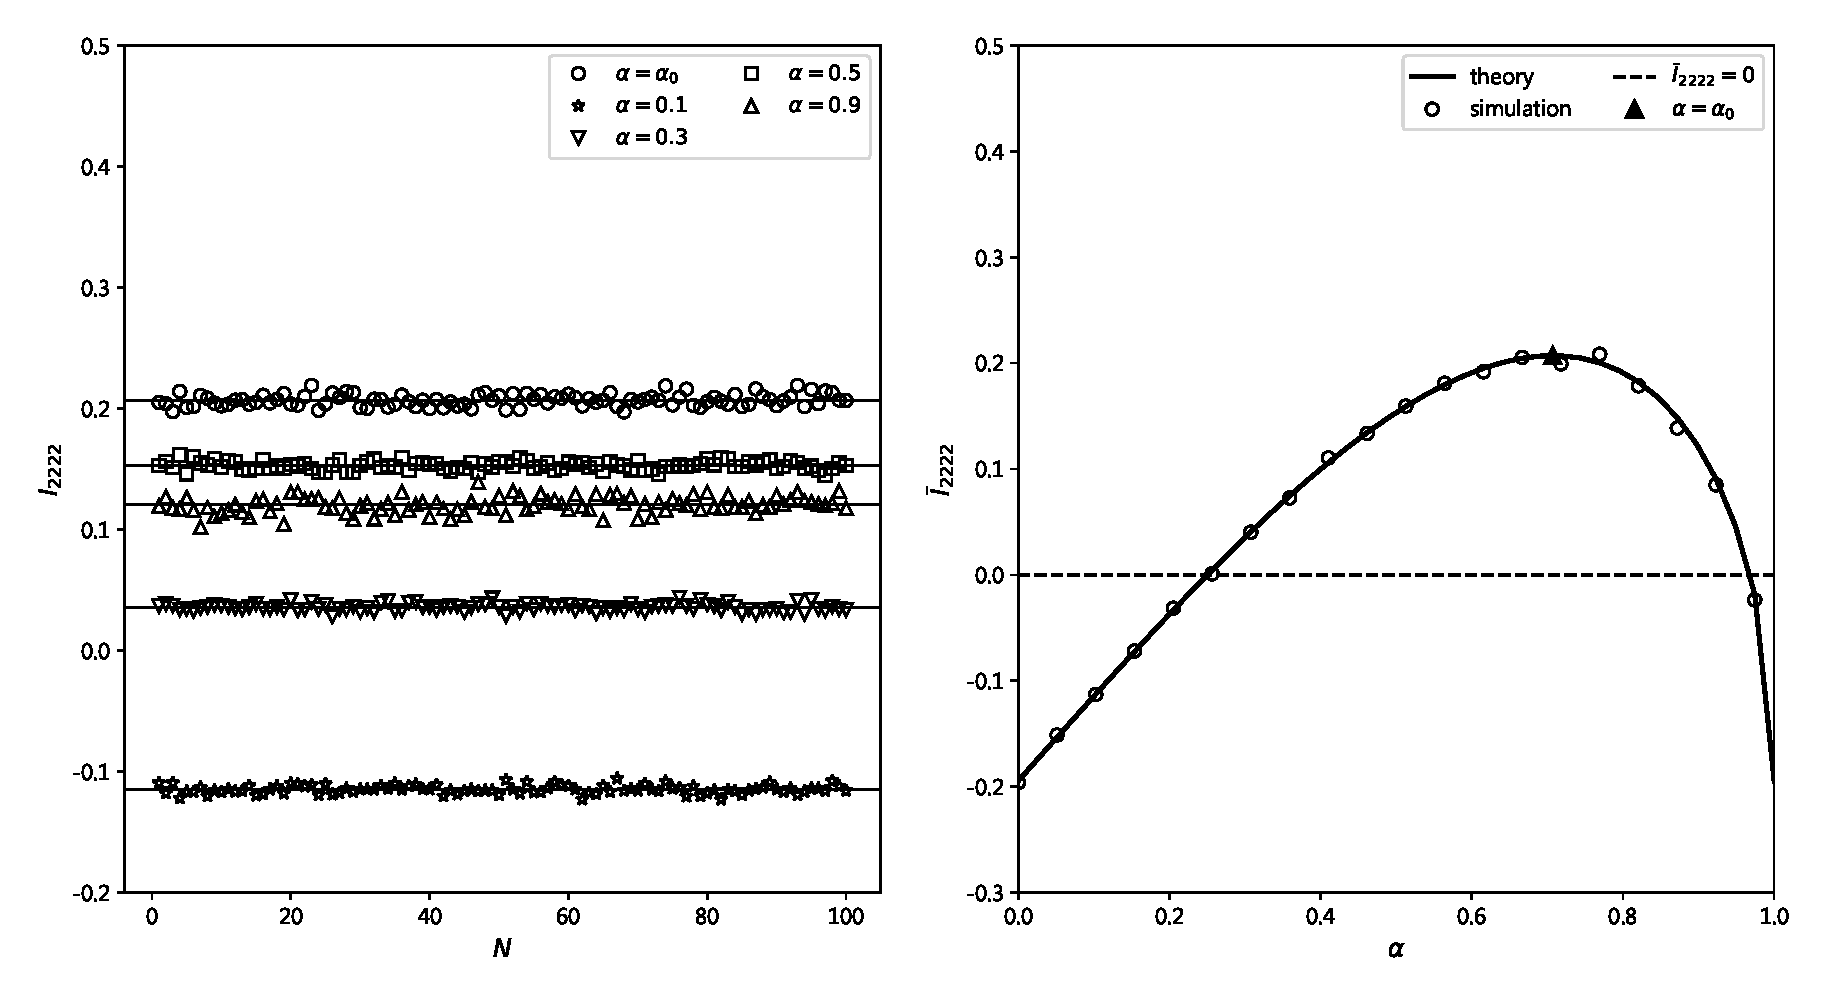
\includegraphics[width=0.76\paperwidth]
    {Datapicture/I2222_figure_1.pdf}%
    }
    \caption{(a) $I_{2222}$ 隨輪數 $N$ 的變化關係；
    (b) $I_{2222}$ 與 $\alpha$ 的關係
    。本研究參考文獻~\protect\cite{CHSH1969} 之理論與參數，自行撰寫程式模擬繪製。}\label{fig:I2222-simulation}
\end{figure}

\begin{figure}[H]
    \makebox[\textwidth][c]{%
    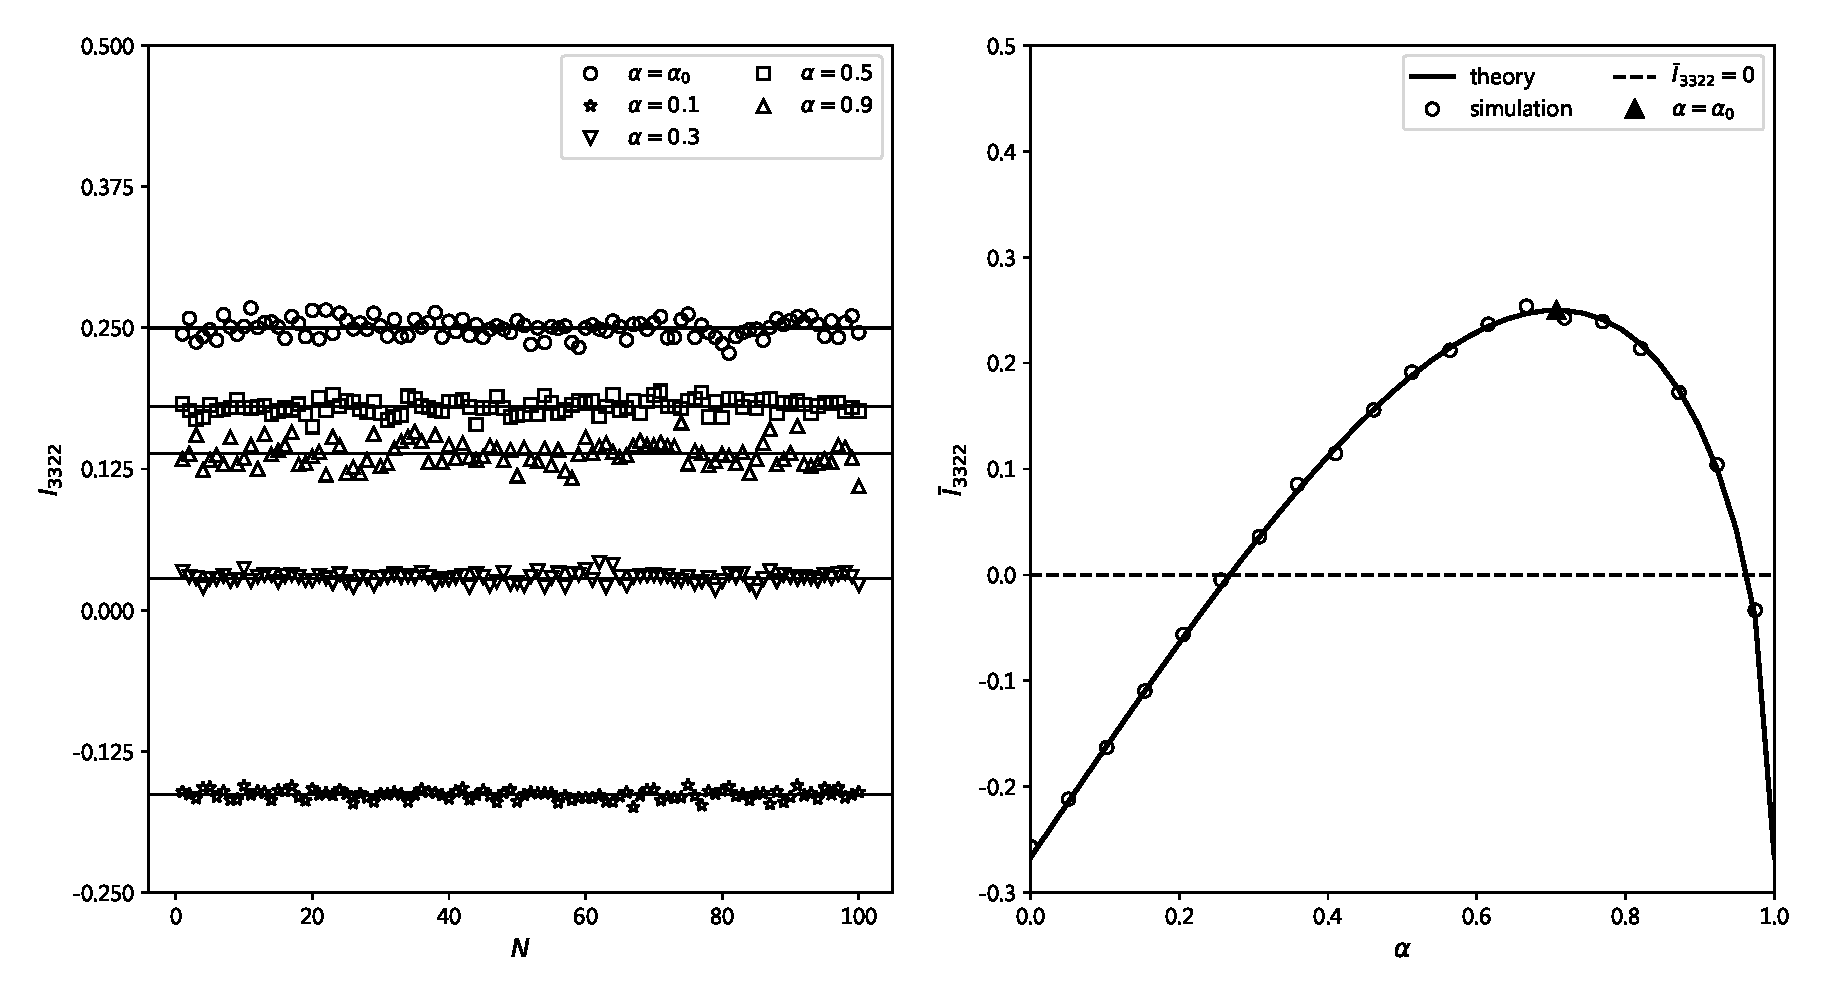
\includegraphics[width=0.76\paperwidth]
    {Datapicture/I3322_figure_1.pdf}%
    }
    \caption{(a) $I_{3322}$ 隨輪數 $N$ 的變化關係；
    (b) $I_{3322}$ 與 $\alpha$ 的關係
    。本研究參考文獻~\protect\cite{Collins2004,Guo2021} 之理論與參數，自行撰寫程式模擬繪製。}\label{fig:I3322-simulation}
\end{figure}

\indent 圖~\ref{fig:I2222-simulation}(a) 與圖~\ref{fig:I3322-simulation}(a)分別顯示$I_{2222}$與 $I_{3322}$在不同$\alpha$下隨機模擬輪數$N$的變化。由結果可觀察到，在固定量子態與測量設定的條件下，各輪模擬值會受到有限取樣所造成的統計漲落影響，因此在相應的理論值附近產生小幅波動；然而整體結果仍維持穩定，且各組模擬平均值皆能良好接近理論預測。
此結果顯示，本文所建立之量子態、投影測量機率與 Bell 不等式計算程序，能夠穩定重現 $I_{2222}$ 與 $I_{3322}$在不同糾纏態下的理論行為，亦可作為後續噪聲模型數值分析之基礎。


\indent 圖~\ref{fig:I2222-simulation}(b) 與圖~\ref{fig:I3322-simulation}(b) 進一步比較$I_{2222}$與 $I_{3322}$隨糾纏數$\alpha$的變化情形。由理論曲線與數值模擬點可觀察到，兩者皆在最大糾纏態$\alpha=\sqrt2/2$附近取得最大的違背值。其中 $I_{2222}$可達$\frac{1}{\sqrt2}-\frac12\approx0.2071$，而$I_{3322}$可達$0.25$，數值模擬結果與前述理論推導具有良好一致性，顯示本文所建立之數值模型能正確重現兩種 Bell 不等式在最大糾纏態附近的量子違背特性。

\noindent 另一方面，當 $\alpha$ 遠離最大糾纏態時，兩種 Bell 不等式的量子違背值皆逐漸下降，並可能在部分參數區域降至局域隱變量模型的上界$I=0$以下。此結果說明，在固定測量設定的條件下，Bell 不等式是否產生量子違背，除了取決於測量方向之外，也與量子態本身的糾纏程度密切相關。換言之，即使量子態本身具有非零糾纏，也不代表在任意固定測量設定下皆必然能夠觀察到 Bell 不等式的違背。

\indent 綜合圖~\ref{fig:I2222-simulation} 與圖~\ref{fig:I3322-simulation} 的結果可知，本文所建立的$I_{2222}$與 $I_{3322}$數值模型均能良好重現相應的理論曲線與最大糾纏態下之量子違背值，顯示理論推導與數值實作具有一致性。

\indent 為進一步比較 $I_{2222}$ 與 $I_{3322}$ 對測量設定的敏感程度，本文將兩種不等式在最大糾纏態下所得到的最佳測量設定互相交換使用。首先，將 $I_{2222}$ 的最佳測量設定$(A_1,~A_2,~B_1,~B_2)$帶入$I_{3322}$中。由於 $I_{3322}$ 在 Alice 與 Bob 兩側各比 $I_{2222}$ 多一組測量設定，因此保留原有四組測量方向後，再針對額外的 $A_3'$ 與 $B_3'$ 進行最佳化，使 $I_{3322}$ 在既有 $I_{2222}$ 測量架構下重新尋找較佳的測量組合。
\begin{figure}[H]
    \centering
    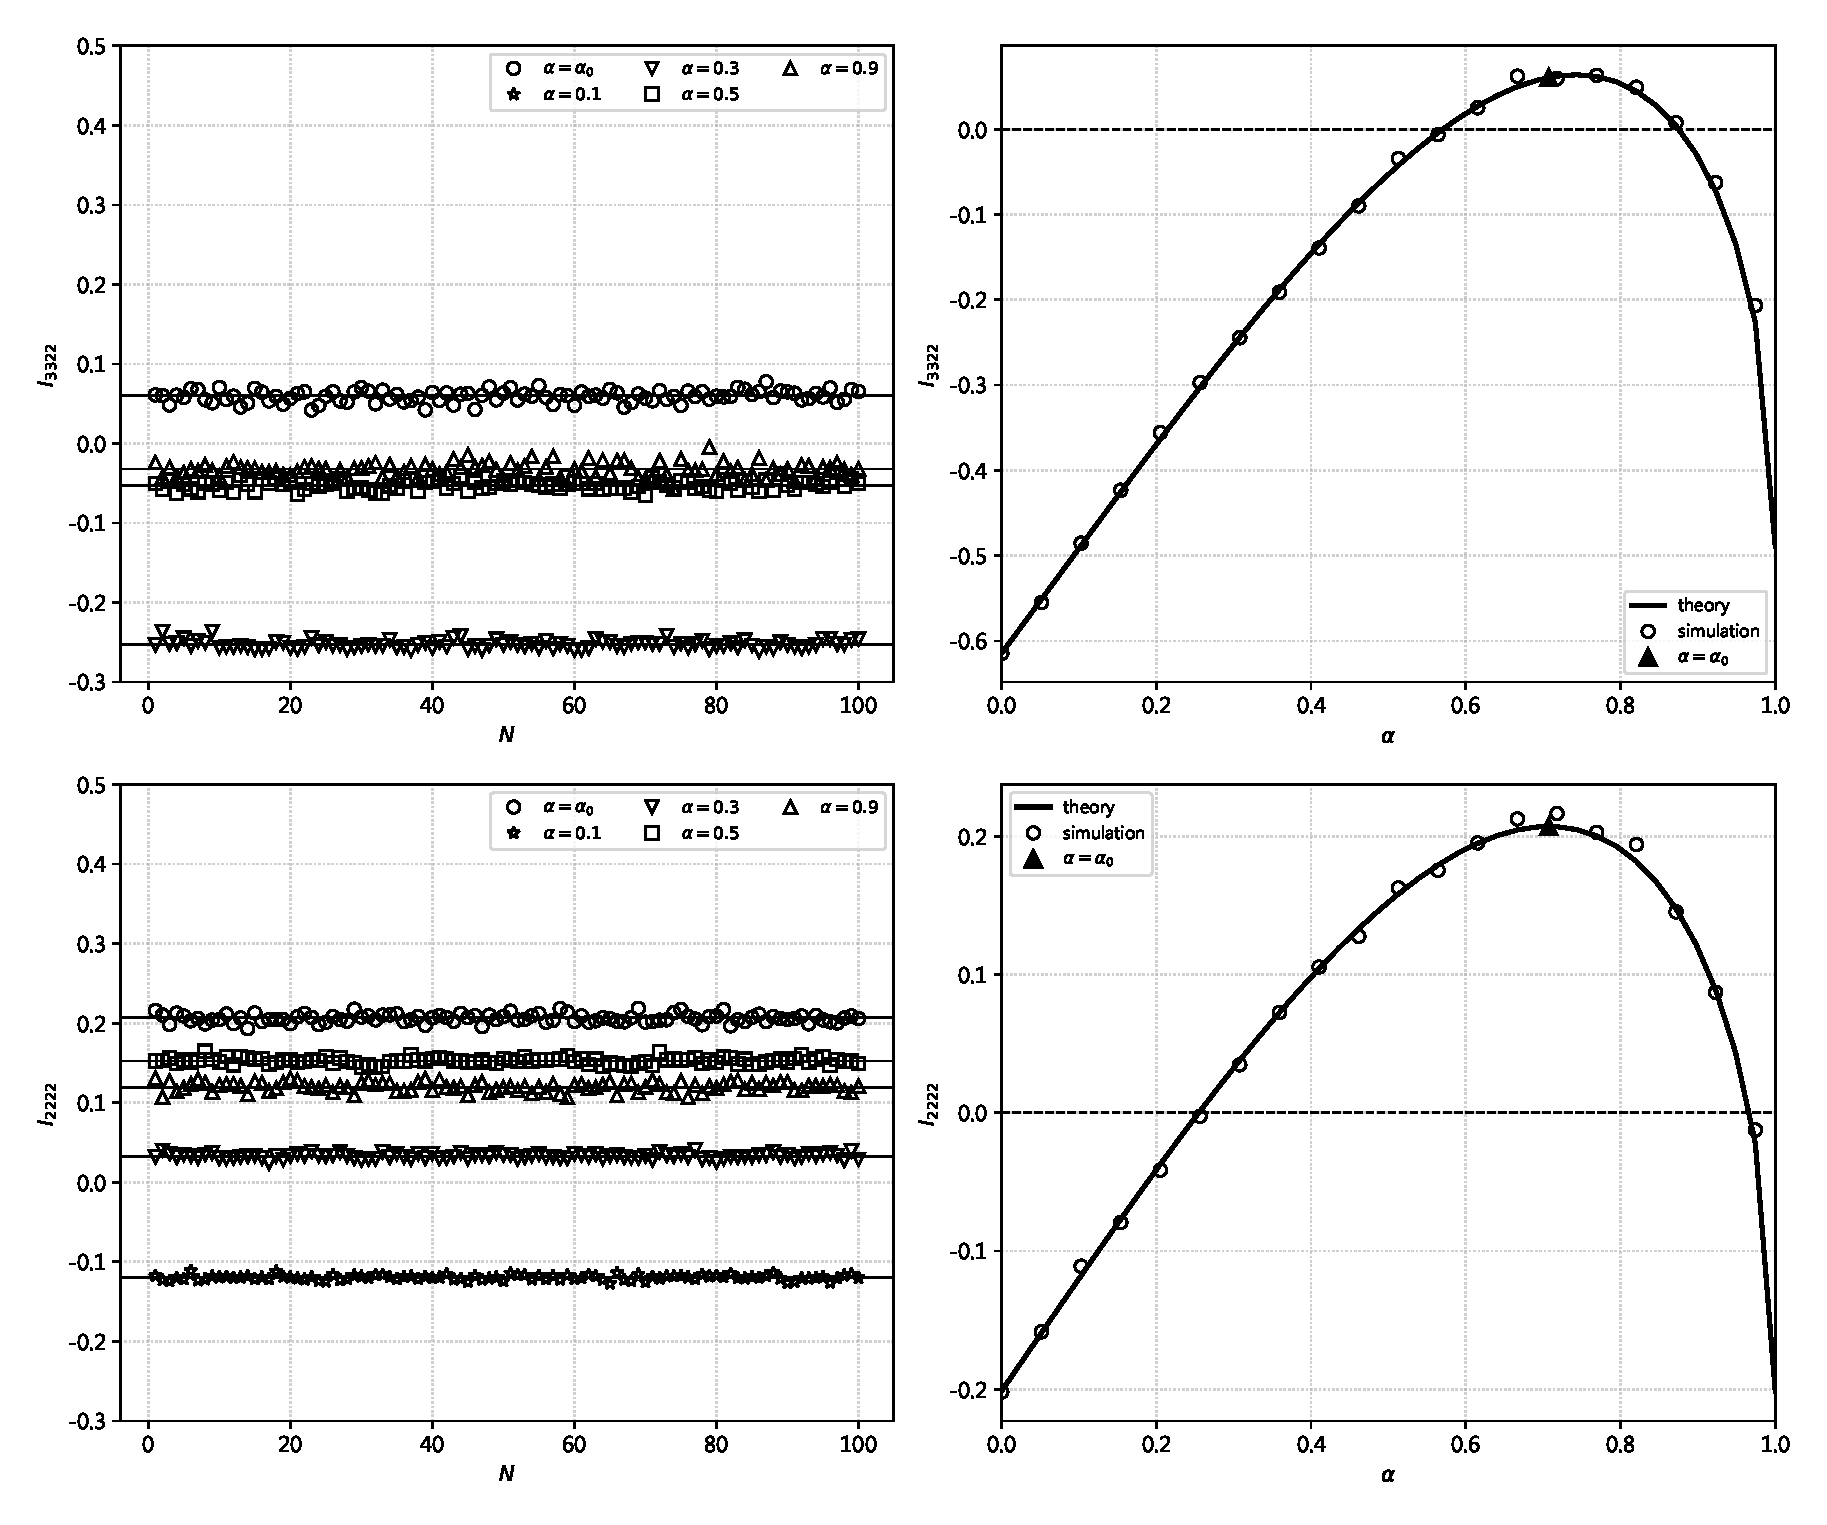
\includegraphics[width=0.90\textwidth]{Datapicture/I2222_to_I3322_figure_1.pdf}
    \caption{$I_{2222}$將最佳測量基設定於$I_{3322}$：上圖為$I_{3322}$、下圖為$I_{2222}$。本研究參考文獻~\protect\cite{CHSH1969,Collins2004,Guo2021} 之理論與參數，自行撰寫程式模擬繪製。}
    \label{fig:I22-to-I32}
\end{figure}
由圖~\ref{fig:I22-to-I32}~可觀察到，即使前四組測量方向原先是針對 $I_{2222}$ 所最佳化，$I_{3322}$ 仍可藉由額外的第三組測量設定調整其聯合機率項，使部分糾纏參數區域仍能產生 Bell 不等式違背。此結果表示，在既有測量方向受到限制的情況下，$I_{3322}$ 額外增加的測量設定提供了更多可調整的自由度。

\indent 相反地，若將 $I_{3322}$ 的最佳測量設定中的前四組$(A_1',~A_2',~B_1',B_2')$帶入$I_{2222}$。
\begin{figure}[H]
    \centering
    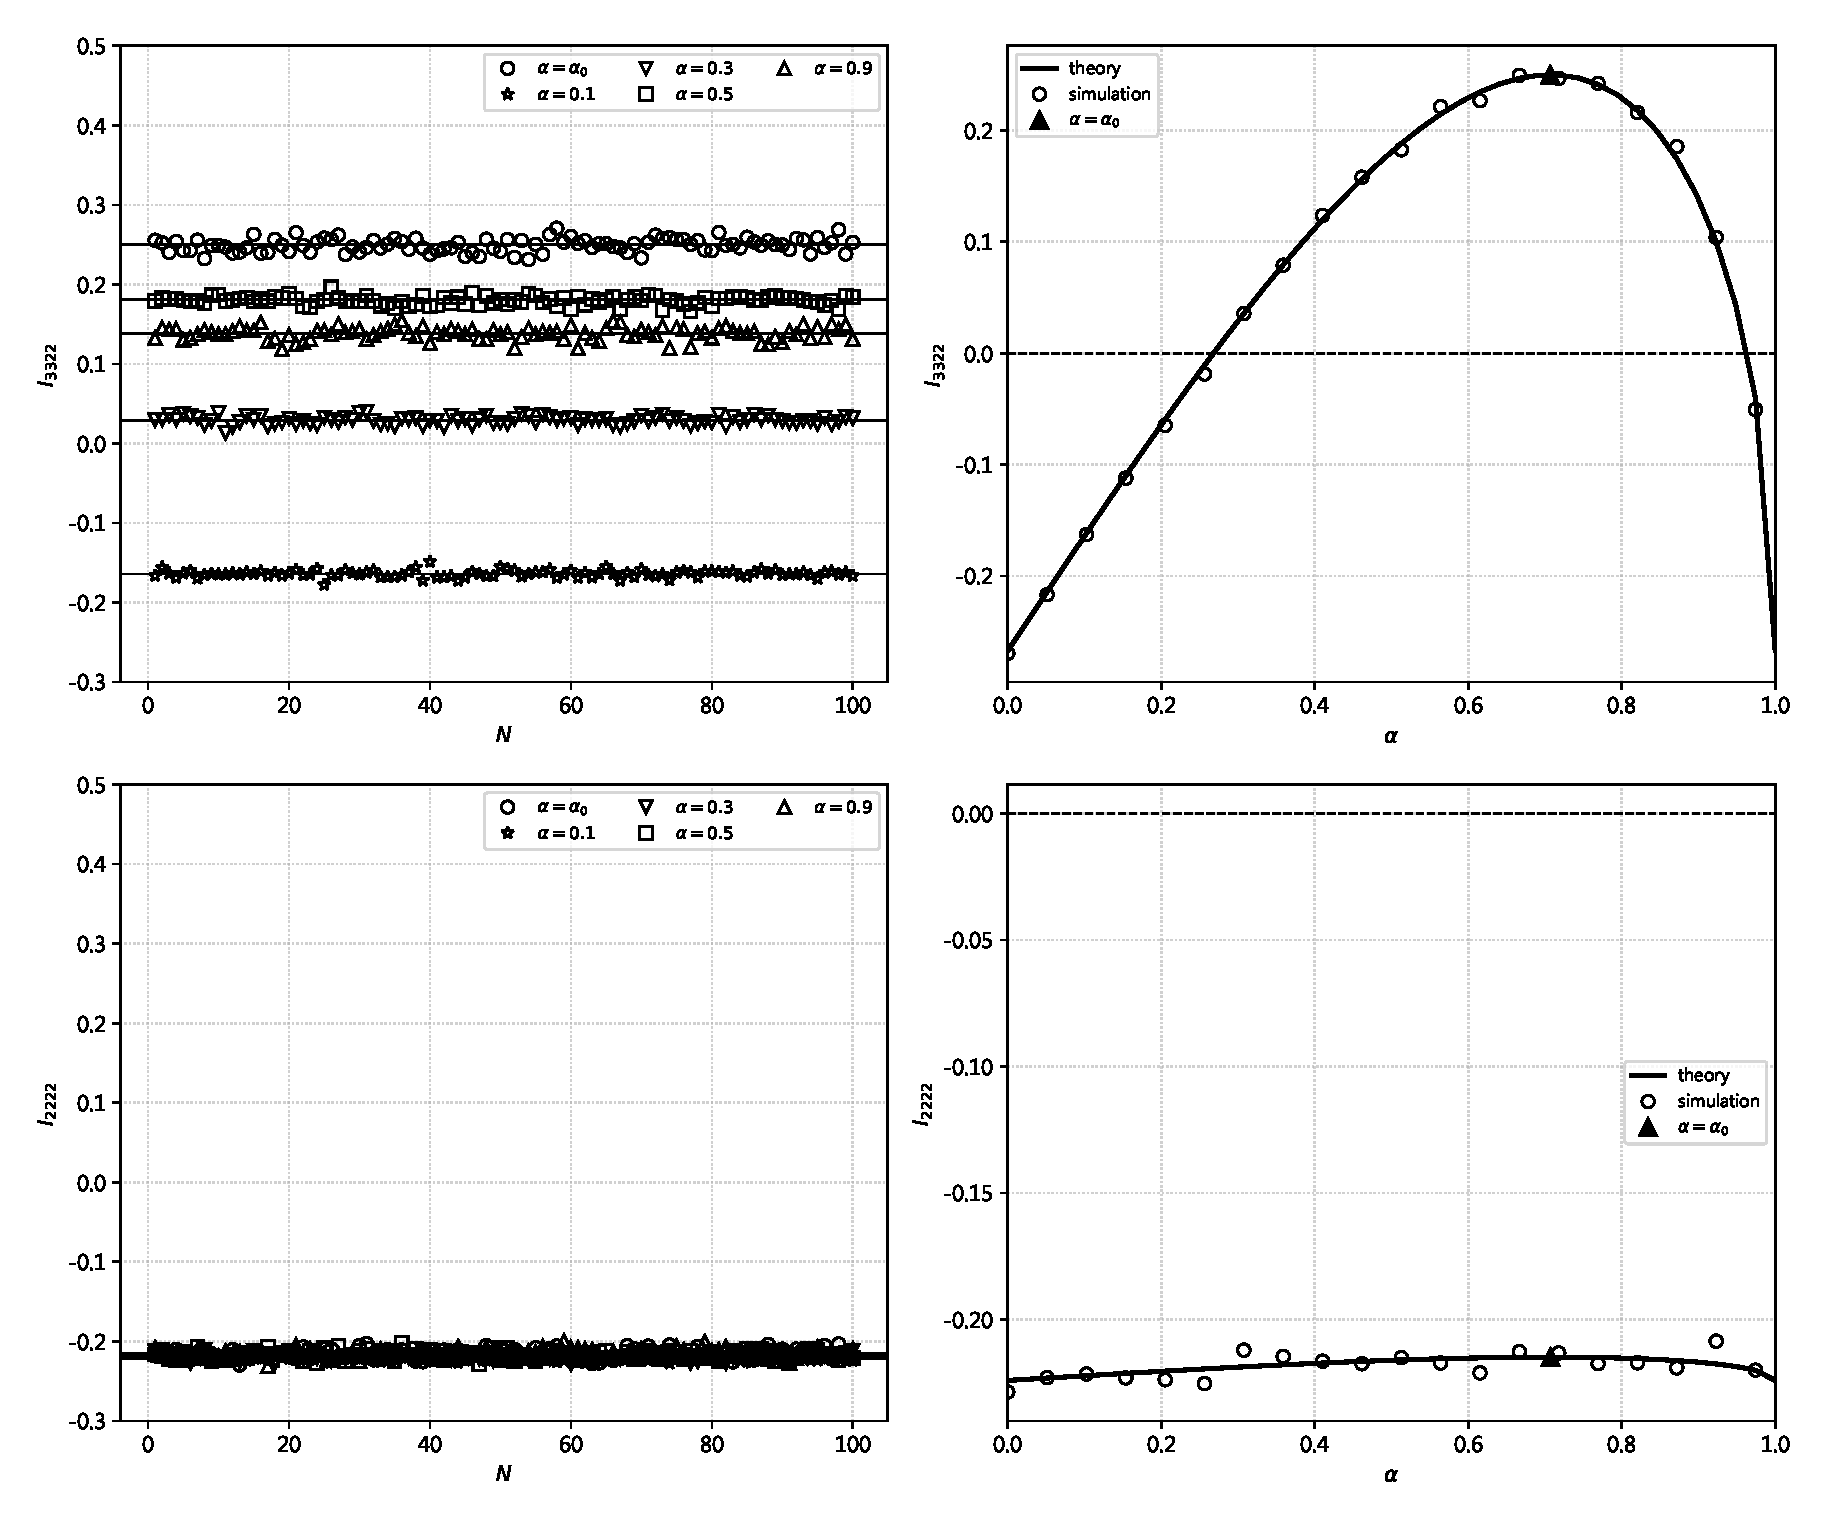
\includegraphics[width=0.90\textwidth]{Datapicture/I3322_to_I2222_figure_1.pdf}
    \caption{$I_{3322}$將最佳測量基設定於$I_{2222}$：上圖為$I_{3322}$、下圖為$I_{2222}$。本研究參考文獻~\protect\cite{CHSH1969,Collins2004,Guo2021} 之理論與參數，自行撰寫程式模擬繪製。}
    \label{fig:I32-to-I22}
\end{figure}
由於$I_{2222}$僅具有兩組測量設定，因此無法再透過額外測量方向進行補償或重新最佳化。由圖~\ref{fig:I32-to-I22}~可觀察到，在此固定測量設定下，$I_{2222}$的違背值明顯受到限制，部分原本可違背$I_{2222}$的量子態，在此設定中已無法超過古典上界。

\indent 上述比較顯示，$I_{3322}$ 因具有較多測量設定，在測量方向受到限制或並非完全最佳的情況下，可能具有較大的調整空間。基於此結果，本文提出以下研究假設：若量子態進一步受到環境噪聲干擾，$I_{3322}$ 是否可能因具有較多測量設定，而在部分噪聲條件下維持較穩定的 Bell 違背。然而，較多的測量設定僅代表最佳化自由度增加，並不能直接推出較高的噪聲抵抗能力。因此，下一節將引入白噪聲與噪聲通道模型，分別觀察 $I_{2222}$ 與 $I_{3322}$ 的違背值隨噪聲參數增加時的變化，並比較兩者違背消失時所對應的臨界參數，以檢驗上述假設是否成立。

\subsection{白噪音對 Bell 不等式量子違背之影響}

在前述純糾纏態分析中，$I_{3322}$ 與 $I_{2222}$ 皆能在最大糾纏態及各自最佳測量設定下取得其最大量子違背值，其中

\[
\begin{aligned}
I_{3322}^{\max}=0.25,\qquad
I_{2222}^{\max}=\frac{1}{\sqrt2}-\frac{1}{2}&\approx 0.2071.
\end{aligned}
\]


\subsubsection{Werner white-noise model}

為描述最大糾纏態受到白噪音干擾後的量子態，本研究依據文獻 \cite{Brunner2008} 採用 Werner state 模型

\begin{equation}
\rho_w
=
w|\Phi^+\rangle\langle\Phi^+|
+
(1-w)\frac{I_4}{4},
\qquad
0\leq w\leq 1.
\end{equation}

\noindent 其中 $w$ 表示最大糾纏態在混合態中所占的比例，而 $1-w$ 則表示白噪音所占的比例。當 $w=1$ 時，系統為未受白噪音影響的最大糾纏態；當 $w=0$ 時，系統則為完全混合態

\[
\rho_0=\frac{I_4}{4}.
\]

\noindent 因此，隨著 $w$ 由 $1$ 逐漸降低，表示系統中所加入的白噪音比例逐漸增加。

\subsubsection{白噪音對關聯函數的影響}

令 Alice 與 Bob 的二元測量 observable 分別表示為
\[
A_i=\bm{a_i}\cdot\bm{\sigma},
\qquad
B_j=\bm{b_j}\cdot\bm{\sigma}.
\]

\noindent 在 Werner state 下，Alice 與 Bob 的關聯函數可表示為
\begin{equation}
E_{ij}(w)
=
\operatorname{Tr}
\left[
\rho_w(A_i\otimes B_j)
\right].
\end{equation}

\noindent 將 Werner state 代入得
\[
\begin{aligned}
E_{ij}(w)
={}&
w\operatorname{Tr}
\left[
|\Phi^+\rangle\langle\Phi^+|
(A_i\otimes B_j)
\right]
\\
&+
\frac{1-w}{4}
\operatorname{Tr}
\left[
I_4(A_i\otimes B_j)
\right].
\end{aligned}
\]

\noindent 由於 $A_i$ 與 $B_j$ 皆由 Pauli matrices 的線性組合所構成，而 Pauli matrices 皆為無跡矩陣，因此
\[
\operatorname{Tr}(A_i)=0,
\qquad
\operatorname{Tr}(B_j)=0.
\]

\noindent 又因為
\[
\operatorname{Tr}(A_i\otimes B_j)
=
\operatorname{Tr}(A_i)\operatorname{Tr}(B_j),
\]

\noindent 故白噪音項滿足
\[
\operatorname{Tr}
\left[
\frac{I_4}{4}(A_i\otimes B_j)
\right]
=0.
\]

\noindent 因此可得
\begin{equation}
E_{ij}(w)=wE_{ij}(1).
\end{equation}

\noindent 由上式可知，Werner white noise 不會額外產生量子關聯，而是使原本最大糾纏態的 correlation 依比例 $w$ 衰減。

\subsubsection{\texorpdfstring{$I_{2222}$}{I2222} 的白噪音臨界值}
由前述理論推導可知
\[
I_{2222}
=
-\frac{1}{2}+\frac{1}{4}S_{2222},
\]

\noindent 且在最大糾纏態及最佳測量設定下
\[
S_{2222}^{\max}=2\sqrt{2}.
\]

\noindent 由於加入白噪音後所有關聯函數皆乘上 $w$，因此
\[
S_{2222}^{\max}(w)=2\sqrt{2}\,w.
\]

\noindent 代回 $I_{2222}$ 可得
\begin{equation}
I_{2222}^{\max}(w)
=
-\frac{1}{2}
+
\frac{\sqrt{2}}{2}w.
\end{equation}

\noindent 當 $I_{2222}(w)=0$ 時定義為違背消失的臨界值，因此
\[
-\frac{1}{2}
+
\frac{\sqrt{2}}{2}w_c
=0,
\]

\noindent 可得
\begin{equation}
w_c^{2222}
=
\frac{1}{\sqrt{2}}
\approx 0.7071.
\end{equation}

\noindent 依據文獻 \cite{Brunner2008} 對 resistance to noise 的定義，可容許的最大白噪音比例為
\begin{equation}
\begin{aligned}
R_{2222}
&=
1-w_c^{2222}\approx 0.2929.
\end{aligned}
\end{equation}

\noindent 因此 $I_{2222}$ 在此條件下約可容許 $29.29\%$ 的白噪音。

\subsubsection{\texorpdfstring{$I_{3322}$}{I3322} 的白噪音臨界值}
同理由前述理論推導可得
\[
I_{3322}
=
-1+\frac{1}{4}S_{3322},
\]

\noindent 且最大糾纏態及最佳測量設定下
\[
S_{3322}^{\max}=5.
\]

\noindent 因此加入 Werner white noise 後
\[
S_{3322}^{\max}(w)=5w.
\]

\noindent 代回 $I_{3322}$：
\begin{equation}
I_{3322}^{\max}(w)
=
-1+\frac{5}{4}w.
\end{equation}

\noindent 則臨界值為$w_c^{3322}=0.8$，因此$I_{3322}$在此條件下可容許$R_{3322}=1-w_c^{3322}=20%$的白噪音。

\begin{figure}[H]
    \centering
    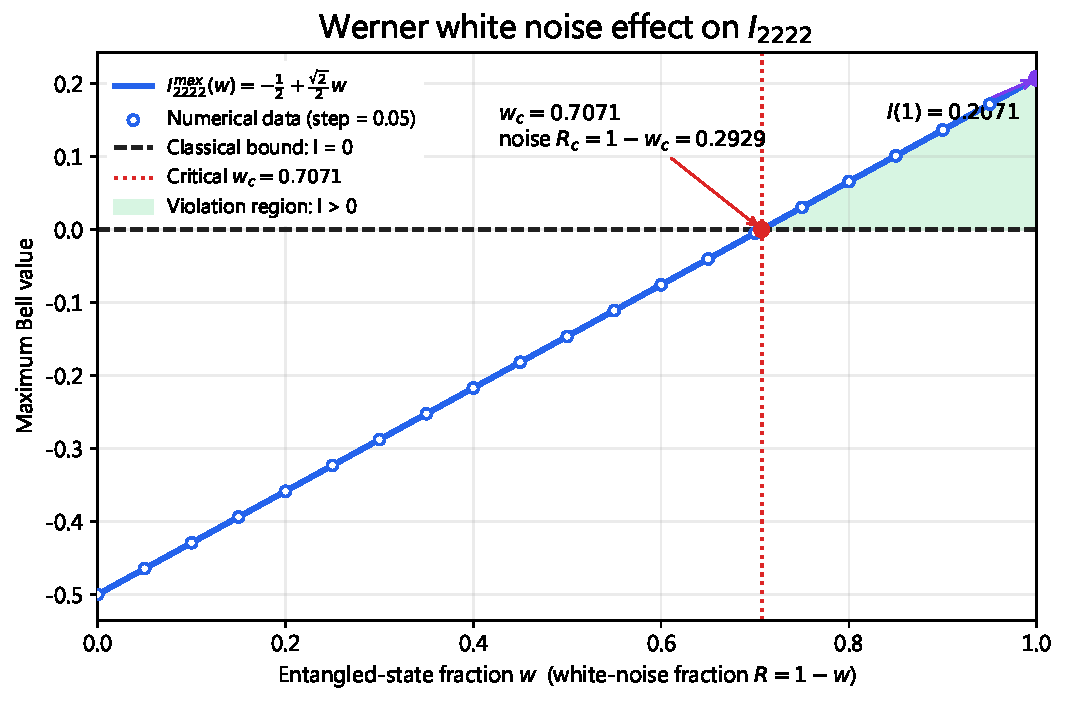
\includegraphics[width=0.78\textwidth]{Datapicture/I2222_vs_w.pdf}
    \par\smallskip
    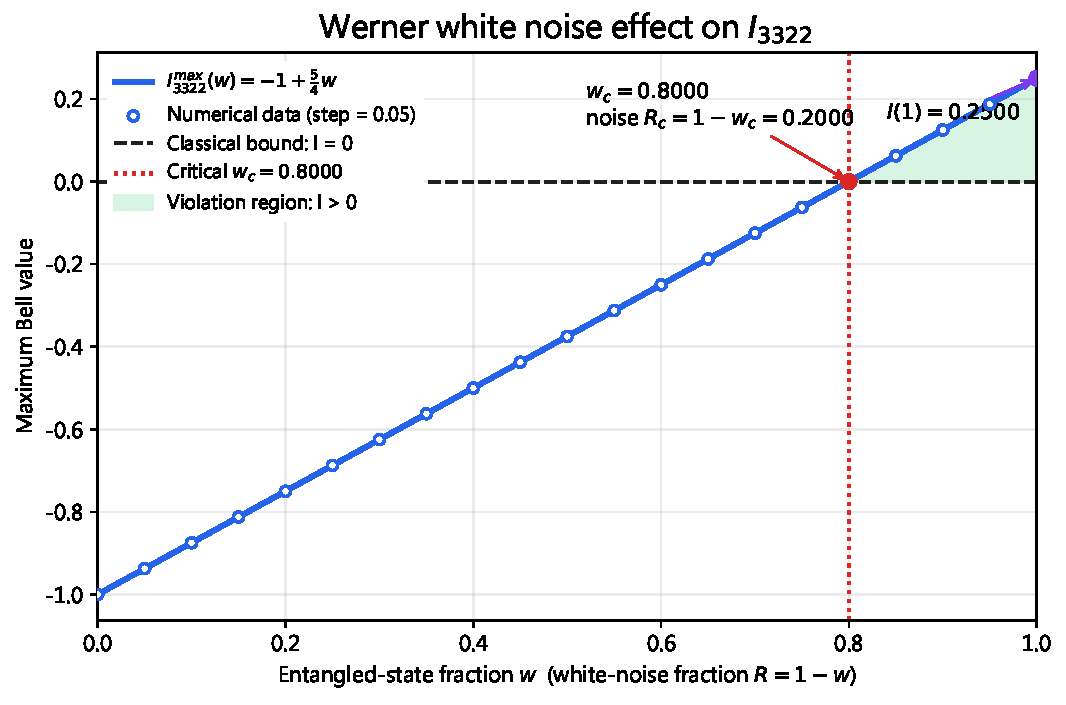
\includegraphics[width=0.78\textwidth]{Datapicture/I3322_vs_w.pdf}
    \caption{$I_{2222}$ 與 $I_{3322}$ 在 Werner white-noise model 下的最大違背值與白噪音臨界值比較：上圖為 $I_{2222}$，下圖為 $I_{3322}$。本研究參考文獻~\protect\cite{Brunner2008} 之理論與參數，自行撰寫程式模擬繪製。}
    \label{fig:werner-white-noise-comparison}
\end{figure}

\noindent 由圖~\ref{fig:werner-white-noise-comparison} 可觀察到，隨著 $w$ 降低，兩種不等式的最大違背值皆逐漸下降。$I_{2222}$ 與 $I_{3322}$ 的臨界值分別為 $w_c=0.7071$ 與 $w_c=0.8000$，對應的白噪音比例分別為 $R_c=0.2929$ 與 $R_c=0.2000$。因此，在本文採用的 Werner white-noise model 與固定最佳測量設定下，$I_{2222}$ 可容許較高比例的白噪音。

\subsection{噪聲通道}

實際上，光子在通道過程中不可避免地要和外界環境相互作用，因此，有必要探討環境噪聲對量子態及 Bell 不等式違背值的影響。一個量子態$\rho$通過噪聲量子通道後的狀態$\rho_{noise}$可表示為$\rho_{noise}=\epsilon(\rho)$，其中 $\epsilon$表示量子通道，可視為作用於密度矩陣上的線性映射。

\noindent 這種描述外部環境對系統影響的量子運算可用 Kraus 算子表示，即
\begin{equation}
    \epsilon(\rho)=\sum_{i}K_i\rho K_i^\dagger
\end{equation}
式中Kraus 算子滿足完備性條件： $\sum_{i}K_i^\dagger K_i=I$。考慮Alice製備糾纏光子對，把其中一個光子通過量子通道發送給Bob的情形，則兩個Kraus 算子表示的噪聲通道可表示為
\begin{equation}
    \rho_{noise}=\sum_{i=1}^{2}(I\otimes K_i)\rho(I\otimes K_i)\dagger
\end{equation}
本文採用文獻中的 two-Kraus-operator channel，其 Kraus 算符可寫為
\begin{equation}
    K_1 = \begin{bmatrix}
        1 & 0\\
        0 & \sqrt{1-p}
    \end{bmatrix},
    \qquad
    K_2 = \begin{bmatrix}
        0 & \eta\sqrt{p}\\
        0 & \sqrt{1-\eta^2}\sqrt{p}
        \end{bmatrix}
\end{equation}
其中 $p\in[0,1]$ 為噪聲強度參數，而 $\eta\in[0,1]$ 則用來調整此模型的型態。當 $p=0$ 時，$K_1=I$且$K_2=0$，因此量子態不受噪聲影響；隨著$p$增加，通道對原始量子態的擾動亦逐漸增強。

\begin{figure}[H]
    \centering
    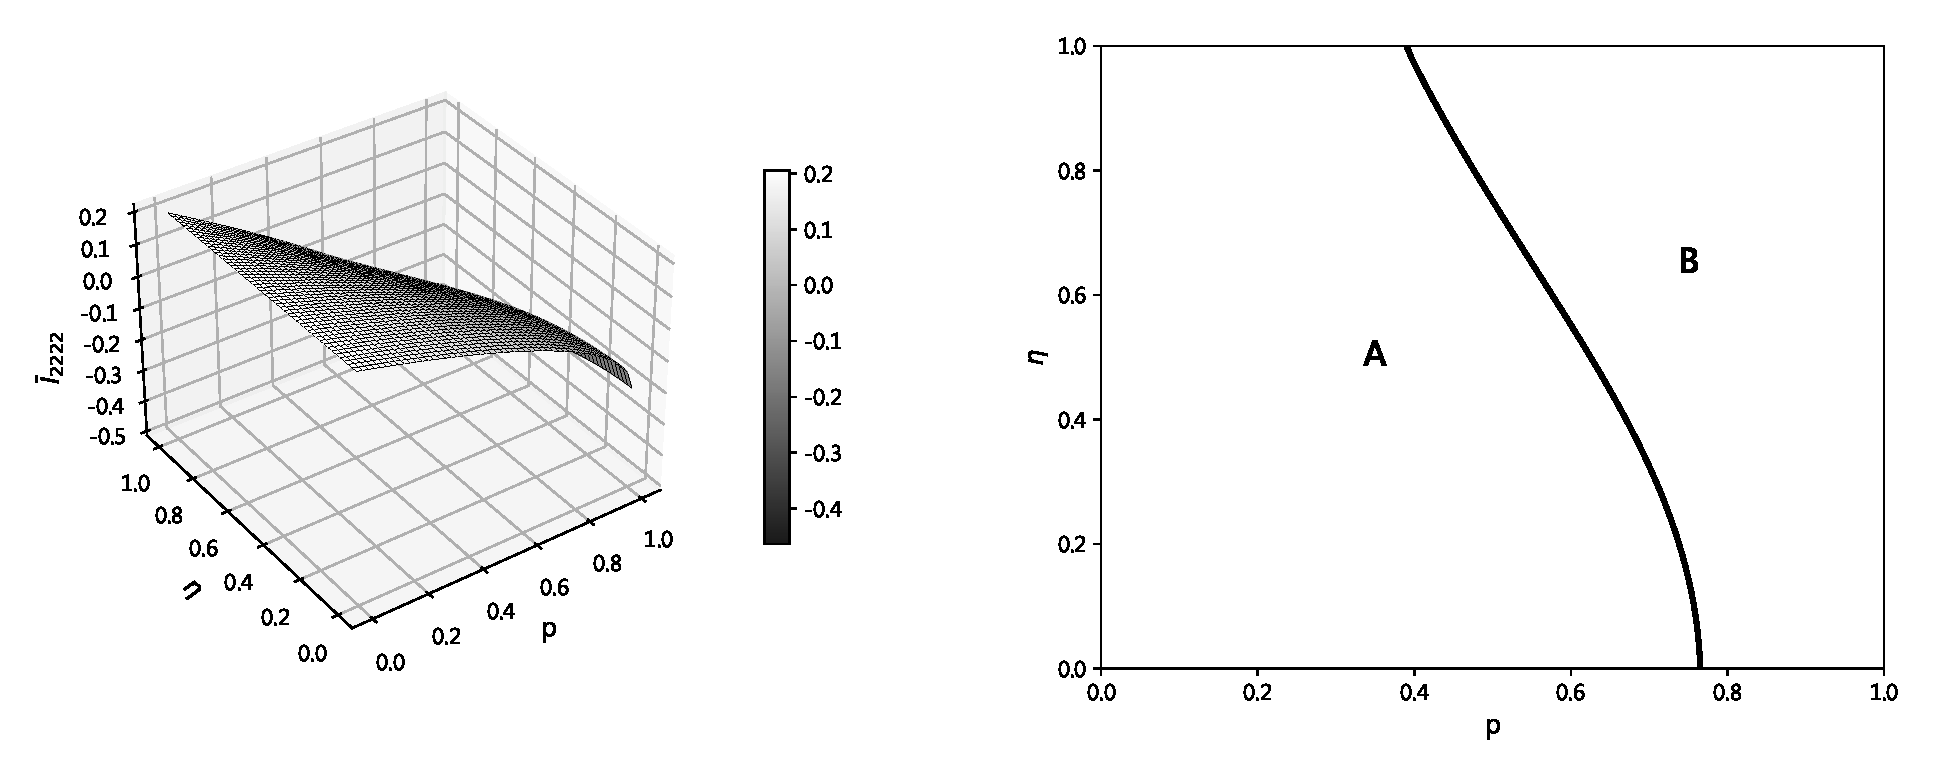
\includegraphics[width=0.60\textwidth]{Datapicture/I2222_figure_3.pdf}
    \par\smallskip
    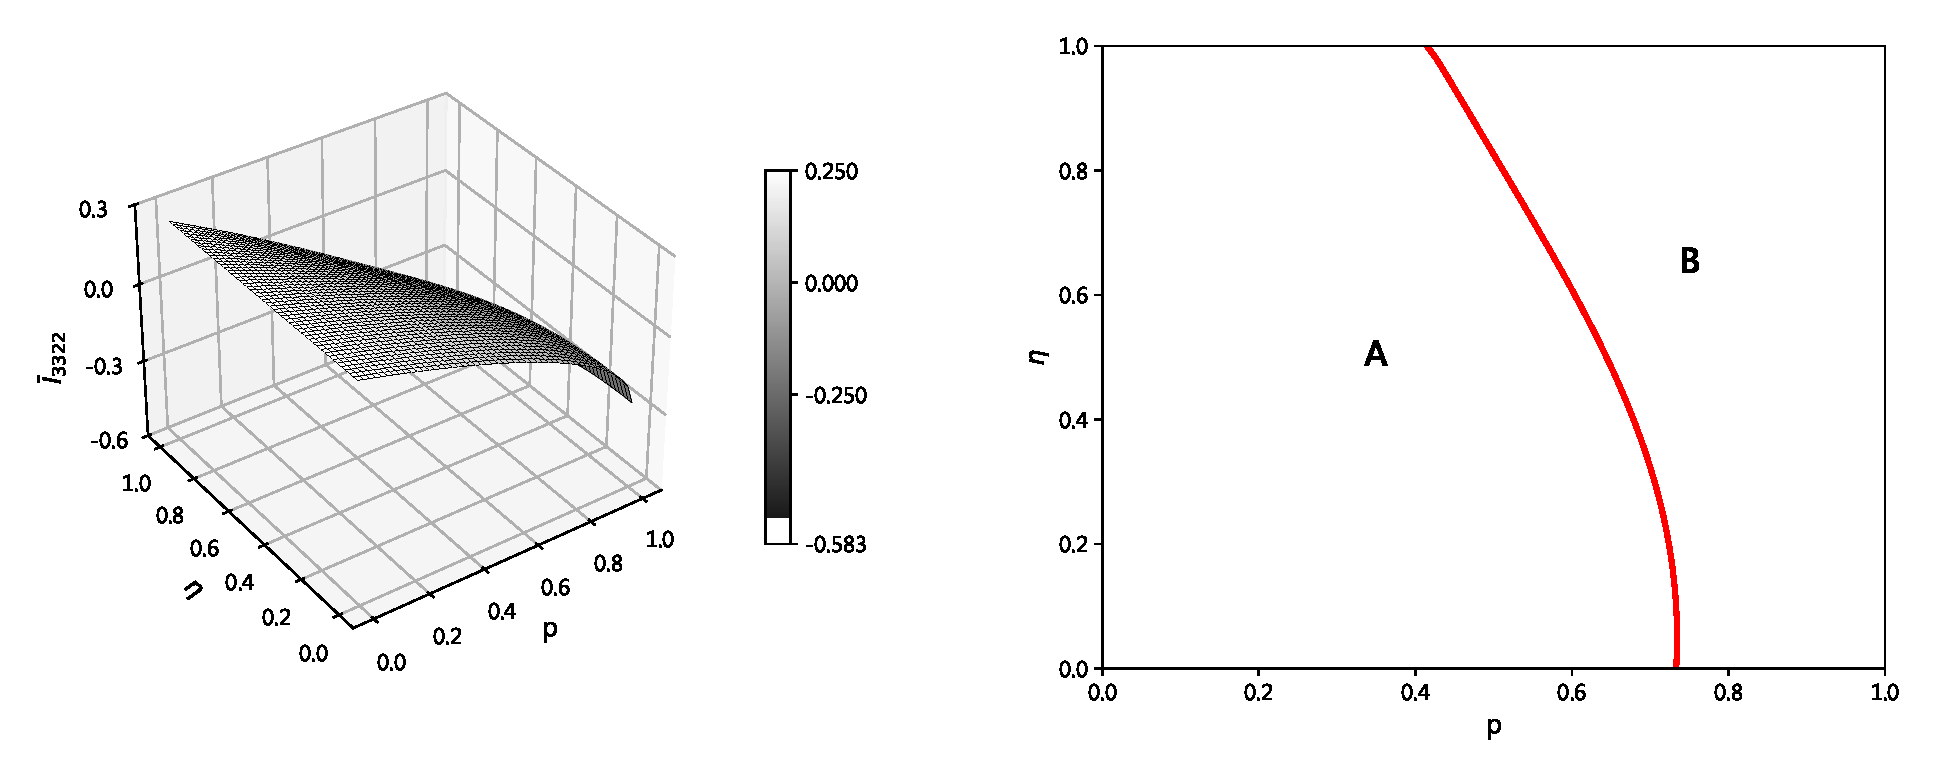
\includegraphics[width=0.60\textwidth]{Datapicture/I3322_figure_3.pdf}
    \caption{$I_{2222}$ 與 $I_{3322}$ 通過噪聲通道的比較：上圖為 $I_{2222}$，下圖為 $I_{3322}$。本研究參考文獻~\protect\cite{Ruan2018} 之噪聲通道參數，自行撰寫程式模擬繪製。}
    \label{fig:noise-boundary-comparison}
\end{figure}

\noindent 其中，將相位圖拿出做比較

\begin{figure}[H]
    \centering
    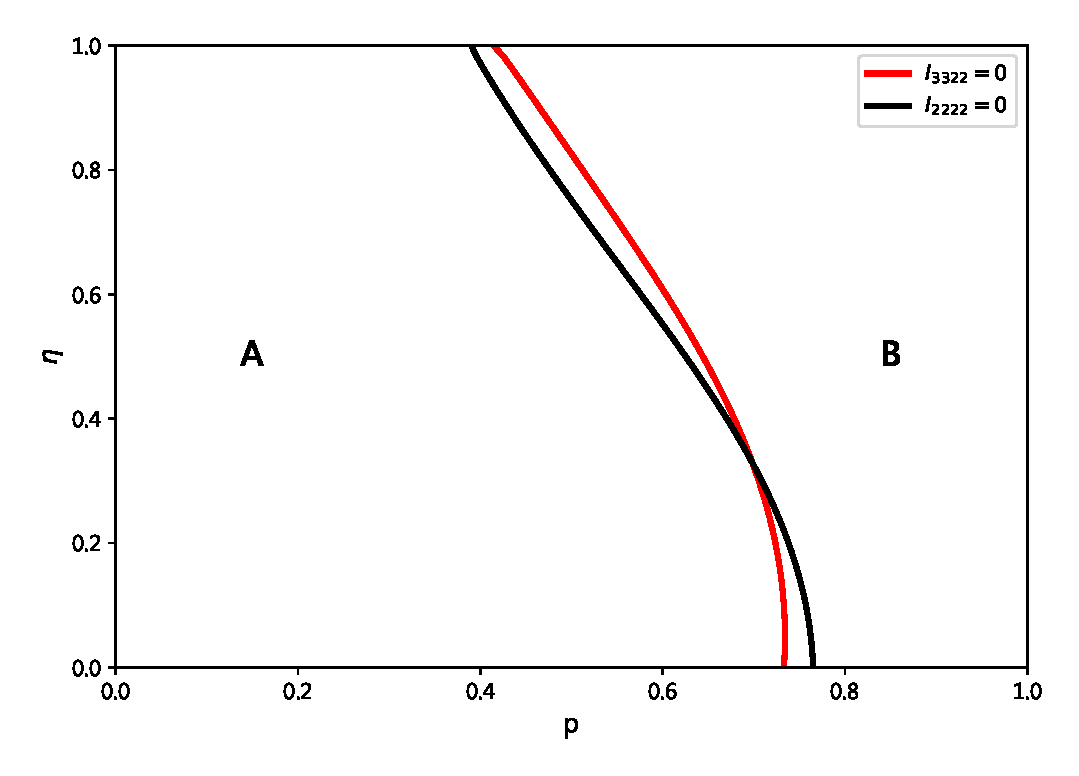
\includegraphics[width=0.8\textwidth]{Datapicture/fixed_angle_noise_figure_3b.pdf}
    \caption{$I_{2222}$ 與 $I_{3322}$ 相位圖比較。本研究參考文獻~\protect\cite{Ruan2018} 之噪聲通道參數，自行撰寫程式模擬繪製。}
    \label{fig:noise-phase}
\end{figure}
由圖~\ref{fig:noise-phase}~可觀察到，$I_{2222}=0$ 與 $I_{3322}=0$兩條臨界曲線將 $(p,\eta)$ 參數空間分成不同區域。其中 A 區表示$I_{2222}>0$ 且 $I_{3322}>0$，亦即兩種 Bell 不等式皆可觀察到違背；B 區則表示$I_{2222}\leq0$ 且 $I_{3322}\leq0$，即兩種不等式皆不再違背古典上界。

\noindent 兩條臨界曲線並未完全重合，因此在其間存在一小段參數區域，使兩種 Bell 不等式對相同噪聲條件產生不同結果。當 $\eta$較大時，可出現$I_{3322}>0$ 且 $I_{2222}\leq0$的情形；而在較低$\eta$的部分區域，則可出現$I_{2222}>0$ 且 $I_{3322}\leq0$的情形。

\noindent 此結果顯示，在本文採用的固定測量設定與噪聲通道下，$I_{3322}$雖具有較多測量設定，但並未在所有噪聲參數下都展現較高的穩健性。兩種不等式的違背區域會隨 $p$ 與 $\eta$ 的不同而改變。

\section{結論}
本文在所採用的雙量子位元最大糾纏態與投影測量架構下，推導 $I_{2222}$ 與 $I_{3322}$ 的古典上界及量子違背，並以 Python 數值模擬檢驗不同糾纏參數下的變化。數值結果與理論推導一致，且兩種 Bell 不等式在各自的最佳測量設定下皆能產生 Bell 違背；其中，$I_{2222}$ 在本文架構下的最大違背值約為 $0.2071$，$I_{3322}$ 的最大違背值為 $0.25$。

\indent 交換最佳測量設定後，兩種不等式呈現不對稱的反應。將 $I_{2222}$ 的最佳測量設定套用至 $I_{3322}$ 時，$I_{3322}$ 因具有額外的第三組測量設定，仍可在前四組測量方向並非自身最佳設定時進行額外最佳化，並對測量方向的不匹配提供一定程度的補償。

\indent 相反地，將 $I_{3322}$ 的前四組最佳測量設定套用至 $I_{2222}$ 時，$I_{2222}$ 沒有額外測量方向可供調整，因此其 Bell 違背範圍受到較明顯的限制。這項比較顯示，額外測量設定所帶來的優勢主要表現在測量方向受限或未達自身最佳設定時的調整空間。

\indent 在 Werner white-noise model 下，本文得到 $I_{2222}$ 與 $I_{3322}$ 的臨界參數分別為 $w_c^{2222}\approx0.7071$ 與 $w_c^{3322}=0.8$，對應的 resistance to noise 分別約為 $0.2929$ 與 $0.2$。在本文採用的量子態與固定測量設定下，$I_{2222}$ 具有較高的白噪聲抵抗能力。此結果說明，較多測量設定或較大的最大量子違背值，均不能直接推出較高的白噪聲穩健性。

\indent 在 two-Kraus-operator channel 中，$I_{2222}=0$ 與 $I_{3322}=0$ 的臨界曲線並未完全重合。於本文所採用的固定測量設定下，部分 $(p,\eta)$ 參數區域會出現 $I_{3322}>0$ 而 $I_{2222}\csname leq\endcsname0$，另一些區域則會出現 $I_{2222}>0$ 而 $I_{3322}\csname leq\endcsname0$。兩種不等式對相同噪聲條件的反應並不完全相同，因而不能將其中一者概括為在所有參數範圍內皆優於另一者。

\indent 在本文採用的量子態、固定測量設定與噪聲模型條件下，較多測量設定確實增加最佳化與調整自由度，但這種自由度不等同於全面較高的噪聲穩健性。比較不同 Bell 不等式時，除了測量設定數量與最大量子違背值之外，亦須同時考慮量子態、測量架構及噪聲模型的具體條件。

% ==============================================================================
%                           引用文獻範例 (Bibliography)
% ==============================================================================
\clearpage
\bibliographystyle{spiebib}% {siamproc}{abbrvnat}% {ksfh_nat}%
\renewcommand{\baselinestretch}{1}
{\small
% [提示]：如果您有獨立的 .bib 檔案，可以保留此行並確保檔名為 Monte_Carlo.bib
\bibliography{references}
}

% 傳統手動輸入文獻預留區 (若不用 .bib 檔，可直接把 \bibitem 取消註解使用)
% \begin{thebibliography}{99}
% \bibitem{Evans-Swartz} M. Evans and T. Swartz, \emph{Approximating Integrals via Monte Carlo}, 2000.
% \bibitem{Wu2021} 武國寧, 孫娜, ``隨機採樣黎曼和,'' \emph{數學傳播}, 2021.
% \bibitem{Caflisch1998} R. E. Caflisch, ``Monte Carlo methods,'' \emph{Acta Numerica}, 1998.
% \end{thebibliography}


% ==============================================================================
%                         英文標題與摘要頁 (完全保留原格式)
% ==============================================================================
\clearpage
\appendix

\section*{附錄一：$I_{2222}$ 數值模擬程式}
\addcontentsline{toc}{section}{附錄一：I2222 數值模擬程式}
本程式用於模擬 $I_{2222}$ 在不同糾纏參數與模擬輪數下的量子違背結果。
\par
程式檔案：\csname texttt\endcsname{I2222simulation.py}

\bigskip
\section*{附錄二：$I_{3322}$ 數值模擬程式}
\addcontentsline{toc}{section}{附錄二：I3322 數值模擬程式}
本程式用於模擬 $I_{3322}$ 在不同糾纏參數與模擬輪數下的量子違背結果。
\par
程式檔案：\csname texttt\endcsname{I3322simulation.py}

\bigskip
\section*{附錄三：$I_{2222}$ 最佳測量設定帶入 $I_{3322}$ 的模擬程式}
\addcontentsline{toc}{section}{附錄三：I2222 最佳測量設定帶入 I3322 的模擬程式}
本程式用於模擬將 $I_{2222}$ 的最佳測量設定帶入 $I_{3322}$ 後的量子違背結果。
\par
程式檔案：\csname texttt\endcsname{I2222toI3322.py}

\bigskip
\section*{附錄四：$I_{3322}$ 最佳測量設定帶入 $I_{2222}$ 的模擬程式}
\addcontentsline{toc}{section}{附錄四：I3322 最佳測量設定帶入 I2222 的模擬程式}
本程式用於模擬將 $I_{3322}$ 的最佳測量設定帶入 $I_{2222}$ 後的量子違背結果。
\par
程式檔案：\csname texttt\endcsname{I3322toI2222.py}
\bigskip

\section*{附錄五：白噪音模擬程式}
\addcontentsline{toc}{section}{附錄五：白噪音模擬程式}
本程式用於模擬 $I_{2222}$ 與 $I_{3322}$ 在 Werner white-noise model 下的最大量子違背值隨參數 $w$ 的變化，並計算兩種不等式的白噪音臨界值。
\par
程式檔案：\csname texttt\endcsname{whitenoise.py}

\clearpage{}
\phantomsection
\renewcommand{\baselinestretch}{1.2}
\vspace*{2cm}

%-----------------------------------------------------------------------
% English Title here
%-----------------------------------------------------------------------
\begin{center}
\textbf{\LARGE
A Study of Bell-Type Inequalities\vspace*{1cm}
}
\par\end{center}

%-----------------------------------------------------------------------
% English authors' information here
%-----------------------------------------------------------------------
{\LARGE \par}
\begin{center}{
\large{LI Shihhong}%
\footnote[1]{\vspace*{-0.5em}
			Corresponding author,  email:S12240005@thu.edu.tw\\
			\hspace*{0.5em} Department of Applied Mathematics, Tunghai University, Taiwan
}
}\par\end{center}
%-----------------------------------------------------------------------
% English Abstract here
%-----------------------------------------------------------------------
\renewcommand{\abstractname}{Abstract}
\renewcommand{\chistory}{\history}
\addcontentsline{toc}{section}{English \abstractname}

\begin{abstract}
Bell inequalities are fundamental tools for testing quantum nonlocality. The $I_{2222}$ inequality\cite{CHSH1969} is a basic Bell-type inequality, whereas $I_{3322}$\cite{Collins2004,Guo2021} adds one measurement setting for each party. Using Python simulations, this study compares their violations for two-qubit pure entangled states, under Werner white noise, and through a two-Kraus-operator channel. The measurement directions are parameterized by Bloch-sphere vectors, and partial differentiation is used to obtain the maximal violations and optimal settings. The simulations agree with the theoretical results. Additional settings allow $I_{3322}$ to retain optimization freedom when the first four directions are not optimal, but do not guarantee greater noise robustness. Under the white-noise model considered here, $I_{2222}$ has the higher resistance to noise, while the two inequalities respond differently in parts of the noisy-channel parameter space.
\medskip{}

%-----------------------------------------------------------------------
% English Keywords here
%-----------------------------------------------------------------------
\noindent \textbf{Keywords:} Bell inequality, quantum nonlocality, quantum noise
\end{abstract}

\csname thispagestyle\endcsname{empty}


\end{document}
